% ***************************************************
% A Classic Thesis Style
% An Homage to The Elements of Typographic Style
%
% Copyright (C) 2012 Andr\'e Miede http://www.miede.de
%
% If you like the style then I would appreciate a postcard. My
% address can be found in the file ClassicThesis.pdf. A collection
% of the postcards I received so far is available online at 
% http://postcards.miede.de
%
% License:
% This program is free software; you can redistribute it and/or
% modify it under the terms of the GNU General Public License as
% published by the Free Software Foundation; either version 2 of
% the License, or (at your option) any later version.
%
% This program is distributed in the hope that it will be useful,
% but WITHOUT ANY WARRANTY; without even the implied warranty of
% MERCHANTABILITY or FITNESS FOR A PARTICULAR PURPOSE.  See the
% GNU General Public License for more details.
%
% You should have received a copy of the GNU General Public
% License along with this program; see the file COPYING.  If not,
% write to the Free Software Foundation, Inc., 59 Temple Place -
% Suite 330, Boston, MA 02111-1307, USA.
%
% ***************************************************************
% Note:
%    * You must not use "u etc. in strings/commands that will be spaced out (use \"u or real umlauts instead)
%    * New enumeration (small caps): \begin{aenumerate} \end{aenumerate}
%    * For margin notes: \marginpar or \graffito{}
%    * Do not use bold fonts in this style, it is designed around them
%    * Use tables as in the examples
%    * See classicthesis-preamble.sty for useful commands
% ****************************************************************

\documentclass[ twoside, 
			openright,
			% letterpaper a4paper
			titlepage, 
			numbers=noenddot,
			headinclude, %1headlines
            		footinclude=true, 
			cleardoublepage=empty,
			abstractoff, % <--- obsolete, remove (todo)
			BCOR=5mm,
			paper=a4, 
			fontsize=11pt, %11pt,
			]{scrreprt}

%*****************************************************************
% Note: Make all your adjustments in here
%*****************************************************************

% \usepackage[backref, backend=biber]{biblatex}
\usepackage[backref,
		backend=bibtex,
            	maxbibnames=99,
            	natbib=true,
            	firstinits=false,
            	style=authoryear-comp,
            	sortcites=false,
            	doi=false,
            	url=false]{biblatex}
\usepackage{lipsum}
\bibliography{Bibliography}	

% ****************************************************************
% classicthesis-config.tex 
% formerly known as loadpackages.sty, classicthesis-ldpkg.sty, and
% classicthesis-preamble.sty Use it at the beginning of your
% ClassicThesis.tex, or as a LaTeX Preamble in your
% ClassicThesis.{tex,lyx} with % ****************************************************************
% classicthesis-config.tex 
% formerly known as loadpackages.sty, classicthesis-ldpkg.sty, and
% classicthesis-preamble.sty Use it at the beginning of your
% ClassicThesis.tex, or as a LaTeX Preamble in your
% ClassicThesis.{tex,lyx} with % ****************************************************************
% classicthesis-config.tex 
% formerly known as loadpackages.sty, classicthesis-ldpkg.sty, and
% classicthesis-preamble.sty Use it at the beginning of your
% ClassicThesis.tex, or as a LaTeX Preamble in your
% ClassicThesis.{tex,lyx} with \input{classicthesis-config}
% ****************************************************************
% If you like the classicthesis, then I would appreciate a
% postcard. My address can be found in the file
% ClassicThesis.pdf. A collection of the postcards I received so
% far is available online at http://postcards.miede.de
% ****************************************************************

% ****************************************************************
% 1. Configure classicthesis for your needs here, e.g., remove
% "drafting" below in order to deactivate the time-stamp on the
% pages
% ****************************************************************
\PassOptionsToPackage{eulerchapternumbers,
					listings,
					%drafting,
				 	pdfspacing,
					floatperchapter,
					%linedheaders,
				 	subfig,
					beramono,
					%eulermath,
					parts}{classicthesis}										

% ****************************************************************
% Triggers for this config
% **************************************************************** 
\usepackage{ifthen}
\newboolean{enable-backrefs} % enable backrefs in the bibliography
\setboolean{enable-backrefs}{false} % true false
% TODO backref is incompatible?
% ****************************************************************


% ****************************************************************
% 2. Personal data and user ad-hoc commands
% ****************************************************************
\newcommand{\myTitle}{Design and Implementation of a Driver\\
for In-Wheel Brushless Motors\\
for Unmanned Vehicles\\\xspace}
\newcommand{\myFirstAuthorName}{Arturo Mont\'ufar Arreola\xspace}
\newcommand{\myMatrFirstAuthor}{840541\xspace}
\newcommand{\mySupervisor}{Prof. Giambattista Gruosso\xspace}
\newcommand{\myOtherSupervisor}{Prof. Luca Bascetta\xspace}
\newcommand{\myExaminer}{Prof. Luigi Piegari\xspace}
\newcommand{\myFaculty}{Facolt\`a di Ingegneria\xspace}
\newcommand{\mySchool}{Scuola di Ingegneria Industriale e dell'Informazione\xspace}
\newcommand{\myDepartment}{Dipartimento di Elettronica, Informazione e Bioingegneria\xspace}
\newcommand{\myCourseFirstPart}{Master of Science in Electronics Engineering\xspace}
\newcommand{\myUni}{Politecnico di Milano\xspace}
\newcommand{\myLocation}{Milan\xspace}
\newcommand{\myTime}{December 2017\xspace}
%\newcommand{\myVersion}{version 1.0\xspace}
\newcommand{\myAcademicYear}{Academic Year 2016-2017\xspace}

% ********************************************************************
% Setup, fine tuning, and useful commands
% ********************************************************************
\newcounter{dummy} % necessary for correct hyperlinks (to index, bib, etc.)
\newlength{\abcd} % for ab..z string length calculation
\providecommand{\mLyX}{L\kern-.1667em\lower.25em\hbox{Y}\kern-.125emX\@}
% from here till the end of the section, you can modify whatever you want
\newcommand{\ie}{i.\,e.\ }
\newcommand{\Ie}{I.\,e.\ }
\newcommand{\eg}{e.\,g.\ }
\newcommand{\Eg}{E.\,g.\ }
% referencing commands
\newcommand{\myEq}[1]{equation \eqref{#1}}
\newcommand{\MyEq}[1]{Equation \eqref{#1}}
\newcommand{\myFig}[1]{figure \ref{#1}}
\newcommand{\MyFig}[1]{Figure \ref{#1}}
\newcommand{\myTab}[1]{table \ref{#1}}
\newcommand{\MyTab}[1]{Table \ref{#1}}
\newcommand{\mySubsec}[1]{subsection \ref{#1}}
\newcommand{\MySubsec}[1]{Subsection \ref{#1}}
\newcommand{\mySec}[1]{section \ref{#1}}
\newcommand{\MySec}[1]{Section \ref{#1}}
\newcommand{\myChap}[1]{chapter \ref{#1}}
\newcommand{\MyChap}[1]{Chapter \ref{#1}}
\newcommand{\myAppendix}[1]{appendix \ref{#1}}
\newcommand{\MyAppendix}[1]{Appendix \ref{#1}}
\newcommand{\myEmph}[1]{\textsc{#1}}

% **********************************************************************


% **********************************************************************
% 3. Loading some handy packages
% **********************************************************************
\PassOptionsToPackage{T1}{fontenc} % T2A for cyrillics
	\usepackage{fontenc} 
\PassOptionsToPackage{utf8}{inputenc} % latin9 (ISO-8859-9) = latin1+"Euro sign"
	\usepackage{inputenc}				

\PassOptionsToPackage{autostyle,italian=guillemets,threshold=1}{csquotes}
 	\usepackage{csquotes}

\PassOptionsToPackage{american,italian}{babel}
	 \usepackage{babel}

\usepackage{textcomp} % fix warning with missing font shapes
\usepackage{scrhack} % fix warnings when using KOMA with listings package          
\usepackage{xspace} % to get the spacing after macros right  
\usepackage{mparhack} % get marginpar right
\usepackage{fixltx2e} % fixes some LaTeX stuff
\usepackage{microtype}
\usepackage[normalem]{ulem} % to have strikethrough text

\PassOptionsToPackage{printonlyused,smaller}{acronym}
	\usepackage{acronym} % nice macros for handling all acronyms in the thesis
% **********************************************************************

%*********************************************************************************
% 3.a Math
%*********************************************************************************
\PassOptionsToPackage{fleqn}{amsmath} % math environments and more by the AMS 
 	\usepackage{amsmath}
 
\usepackage{amsthm}
\usepackage{amssymb}
\usepackage{gensymb}
\renewcommand\qedsymbol{$\blacksquare$}

\theoremstyle{definition}
\newtheorem{definition}{Definition}[chapter]
\newtheorem{theorem}{Theorem}[chapter]

\theoremstyle{plain}
\newtheorem{observation}[definition]{Observation}
\newtheorem{corollary}[theorem]{Corollary}
\newtheorem{lemma}[theorem]{Lemma}
% **********************************************************************


% **********************************************************************
% 4. Setup floats: tables, (sub)figures, and captions
% **********************************************************************
\usepackage{tabularx} % better tables
	\setlength{\extrarowheight}{3pt} % increase table row height
\newcommand{\tableheadline}[2]{\multicolumn{1}{#1}{\normalsize\spacedlowsmallcaps{#2}}}
\newcommand{\tableheadlineMore}[3]{\multicolumn{#1}{#2}{\normalsize\spacedlowsmallcaps{#3}}}
\newcommand{\tablefirstcol}[2]{\multicolumn{1}{#1}{\textbf{#2}}}

\usepackage{caption}
	\captionsetup{format=hang,labelfont={sf,bf},font=small}
\usepackage{colortbl}
\usepackage{multirow}

\usepackage{subfig}
\usepackage{siunitx}
% *********************************************************************


% *********************************************************************
% 5. Setup code listings
% *********************************************************************
\usepackage{listings}
\lstloadlanguages{bash, C++, Java, Matlab}

% for special keywords
\lstset{language=[LaTeX]Tex,
    keywordstyle=\color{RoyalBlue},%\bfseries,
    basicstyle=\small\ttfamily,
    %identifierstyle=\color{NavyBlue},
    commentstyle=\color{Green}\ttfamily,
    stringstyle=\rmfamily,
    numbers=none,%left,%
    numberstyle=\scriptsize,%\tiny
    stepnumber=5,
    numbersep=8pt,
    showstringspaces=false,
    breaklines=true,
    frameround=ftff,
    frame=single,
    belowcaptionskip=.75\baselineskip
    %frame=L
} 
% *********************************************************************


% *********************************************************************
% 6. PDFLaTeX, hyperreferences and citation backreferences
% *********************************************************************
% ********************************************************************
% Using PDFLaTeX
% ********************************************************************
\PassOptionsToPackage{pdftex,hyperfootnotes=false,pdfpagelabels}{hyperref}
	\usepackage{hyperref}  % backref linktocpage pagebackref
\pdfcompresslevel=9
\pdfadjustspacing=1 
\PassOptionsToPackage{pdftex}{graphicx}
	\usepackage{graphicx} 

% ********************************************************************
% Setup the style of the backrefs from the bibliography
% (translate the options to any language you use)
% ********************************************************************
\newcommand{\backrefnotcitedstring}{\relax}%(Not cited.)
\newcommand{\backrefcitedsinglestring}[1]{(Cited on page~#1.)}
\newcommand{\backrefcitedmultistring}[1]{(Cited on pages~#1.)}
\ifthenelse{\boolean{enable-backrefs}}%
{%
		\PassOptionsToPackage{hyperpageref}{backref}
		\usepackage{backref} % to be loaded after hyperref package 
		   \renewcommand{\backreftwosep}{ and~} % separate 2 pages
		   \renewcommand{\backreflastsep}{, and~} % separate last of longer list
		   \renewcommand*{\backref}[1]{}  % disable standard
		   \renewcommand*{\backrefalt}[4]{% detailed backref
		      \ifcase #1 %
		         \backrefnotcitedstring%
		      \or%
		         \backrefcitedsinglestring{#2}%
		      \else%
		         \backrefcitedmultistring{#2}%
		      \fi}%
}{\relax}    


% ****************************************************************
% PDF/A compliance
% ****************************************************************
% TODO not working: requires downloading color specification file in a specific
% tex folder and other hacks I don't want to spend time with
% \usepackage[a-1b]{pdfx}

% ********************************************************************
% Hyperreferences
% ********************************************************************
\hypersetup{%
    %draft,	% = no hyperlinking at all (useful in b/w printouts)
    colorlinks=true, linktocpage=true, pdfstartpage=3, pdfstartview=FitV,%
    % uncomment the following line if you want to have black links (e.g., for printing)
    %colorlinks=false, linktocpage=false, pdfborder={0 0 0}, pdfstartpage=3, pdfstartview=FitV,% 
    breaklinks=true, pdfpagemode=UseNone, pageanchor=true, pdfpagemode=UseOutlines,%
    plainpages=false, bookmarksnumbered, bookmarksopen=true, bookmarksopenlevel=1,%
    hypertexnames=true, pdfhighlight=/O,%nesting=true,%frenchlinks,%
    urlcolor=webbrown, linkcolor=RoyalBlue, citecolor=webgreen, %pagecolor=RoyalBlue,%
    %urlcolor=Black, linkcolor=Black, citecolor=Black, %pagecolor=Black,%
} 

    %pdftitle={\myTitle},%
    %pdfauthor={\textcopyright\ \myFirstAuthorName and \mySecondAuthorName, \myUni, \myFaculty},%
    %pdfsubject={},%
    %pdfkeywords={},%
    %pdfcreator={pdfLaTeX},%
    %pdfproducer={LaTeX with hyperref and classicthesis}%

%}   

% ********************************************************************
% Setup autoreferences
% ********************************************************************
% There are some issues regarding autorefnames
% http://www.ureader.de/msg/136221647.aspx
% http://www.tex.ac.uk/cgi-bin/texfaq2html?label=latexwords
% you have to redefine the makros for the 
% language you use, e.g., american, ngerman
% (as chosen when loading babel/AtBeginDocument)
% ********************************************************************
\makeatletter
\@ifpackageloaded{babel}%
    {%
       \addto\extrasamerican{%
					\renewcommand*{\figureautorefname}{Figure}%
					\renewcommand*{\tableautorefname}{Table}%
					\renewcommand*{\partautorefname}{Part}%
					\renewcommand*{\chapterautorefname}{Chapter}%
					\renewcommand*{\sectionautorefname}{Section}%
					\renewcommand*{\subsectionautorefname}{Section}%
					\renewcommand*{\subsubsectionautorefname}{Section}% 	
				}%
       \addto\extrasitalian{% 
					\renewcommand*{\paragraphautorefname}{Paragrafo}%
					\renewcommand*{\subparagraphautorefname}{Paragrafo}%
					\renewcommand*{\footnoteautorefname}{Nota a pié di pagina}%
					\renewcommand*{\FancyVerbLineautorefname}{Zeile}%
					\renewcommand*{\theoremautorefname}{Teorema}%
					\renewcommand*{\appendixautorefname}{Appendice}%
					\renewcommand*{\equationautorefname}{Equazione}%        
					\renewcommand*{\itemautorefname}{Punto}%
				}%	
			% Fix to getting autorefs for subfigures right (thanks to Belinda Vogt for changing the definition)
			\providecommand{\subfigureautorefname}{\figureautorefname}%  			
    }{\relax}
\makeatother

% ****************************************************************
% 7. Last calls before the bar closes
% ****************************************************************

\usepackage{classicthesis} 

% ****************************************************************
% ****************************************************************
% If you like the classicthesis, then I would appreciate a
% postcard. My address can be found in the file
% ClassicThesis.pdf. A collection of the postcards I received so
% far is available online at http://postcards.miede.de
% ****************************************************************

% ****************************************************************
% 1. Configure classicthesis for your needs here, e.g., remove
% "drafting" below in order to deactivate the time-stamp on the
% pages
% ****************************************************************
\PassOptionsToPackage{eulerchapternumbers,
					listings,
					%drafting,
				 	pdfspacing,
					floatperchapter,
					%linedheaders,
				 	subfig,
					beramono,
					%eulermath,
					parts}{classicthesis}										

% ****************************************************************
% Triggers for this config
% **************************************************************** 
\usepackage{ifthen}
\newboolean{enable-backrefs} % enable backrefs in the bibliography
\setboolean{enable-backrefs}{false} % true false
% TODO backref is incompatible?
% ****************************************************************


% ****************************************************************
% 2. Personal data and user ad-hoc commands
% ****************************************************************
\newcommand{\myTitle}{Design and Implementation of a Driver\\
for In-Wheel Brushless Motors\\
for Unmanned Vehicles\\\xspace}
\newcommand{\myFirstAuthorName}{Arturo Mont\'ufar Arreola\xspace}
\newcommand{\myMatrFirstAuthor}{840541\xspace}
\newcommand{\mySupervisor}{Prof. Giambattista Gruosso\xspace}
\newcommand{\myOtherSupervisor}{Prof. Luca Bascetta\xspace}
\newcommand{\myExaminer}{Prof. Luigi Piegari\xspace}
\newcommand{\myFaculty}{Facolt\`a di Ingegneria\xspace}
\newcommand{\mySchool}{Scuola di Ingegneria Industriale e dell'Informazione\xspace}
\newcommand{\myDepartment}{Dipartimento di Elettronica, Informazione e Bioingegneria\xspace}
\newcommand{\myCourseFirstPart}{Master of Science in Electronics Engineering\xspace}
\newcommand{\myUni}{Politecnico di Milano\xspace}
\newcommand{\myLocation}{Milan\xspace}
\newcommand{\myTime}{December 2017\xspace}
%\newcommand{\myVersion}{version 1.0\xspace}
\newcommand{\myAcademicYear}{Academic Year 2016-2017\xspace}

% ********************************************************************
% Setup, fine tuning, and useful commands
% ********************************************************************
\newcounter{dummy} % necessary for correct hyperlinks (to index, bib, etc.)
\newlength{\abcd} % for ab..z string length calculation
\providecommand{\mLyX}{L\kern-.1667em\lower.25em\hbox{Y}\kern-.125emX\@}
% from here till the end of the section, you can modify whatever you want
\newcommand{\ie}{i.\,e.\ }
\newcommand{\Ie}{I.\,e.\ }
\newcommand{\eg}{e.\,g.\ }
\newcommand{\Eg}{E.\,g.\ }
% referencing commands
\newcommand{\myEq}[1]{equation \eqref{#1}}
\newcommand{\MyEq}[1]{Equation \eqref{#1}}
\newcommand{\myFig}[1]{figure \ref{#1}}
\newcommand{\MyFig}[1]{Figure \ref{#1}}
\newcommand{\myTab}[1]{table \ref{#1}}
\newcommand{\MyTab}[1]{Table \ref{#1}}
\newcommand{\mySubsec}[1]{subsection \ref{#1}}
\newcommand{\MySubsec}[1]{Subsection \ref{#1}}
\newcommand{\mySec}[1]{section \ref{#1}}
\newcommand{\MySec}[1]{Section \ref{#1}}
\newcommand{\myChap}[1]{chapter \ref{#1}}
\newcommand{\MyChap}[1]{Chapter \ref{#1}}
\newcommand{\myAppendix}[1]{appendix \ref{#1}}
\newcommand{\MyAppendix}[1]{Appendix \ref{#1}}
\newcommand{\myEmph}[1]{\textsc{#1}}

% **********************************************************************


% **********************************************************************
% 3. Loading some handy packages
% **********************************************************************
\PassOptionsToPackage{T1}{fontenc} % T2A for cyrillics
	\usepackage{fontenc} 
\PassOptionsToPackage{utf8}{inputenc} % latin9 (ISO-8859-9) = latin1+"Euro sign"
	\usepackage{inputenc}				

\PassOptionsToPackage{autostyle,italian=guillemets,threshold=1}{csquotes}
 	\usepackage{csquotes}

\PassOptionsToPackage{american,italian}{babel}
	 \usepackage{babel}

\usepackage{textcomp} % fix warning with missing font shapes
\usepackage{scrhack} % fix warnings when using KOMA with listings package          
\usepackage{xspace} % to get the spacing after macros right  
\usepackage{mparhack} % get marginpar right
\usepackage{fixltx2e} % fixes some LaTeX stuff
\usepackage{microtype}
\usepackage[normalem]{ulem} % to have strikethrough text

\PassOptionsToPackage{printonlyused,smaller}{acronym}
	\usepackage{acronym} % nice macros for handling all acronyms in the thesis
% **********************************************************************

%*********************************************************************************
% 3.a Math
%*********************************************************************************
\PassOptionsToPackage{fleqn}{amsmath} % math environments and more by the AMS 
 	\usepackage{amsmath}
 
\usepackage{amsthm}
\usepackage{amssymb}
\usepackage{gensymb}
\renewcommand\qedsymbol{$\blacksquare$}

\theoremstyle{definition}
\newtheorem{definition}{Definition}[chapter]
\newtheorem{theorem}{Theorem}[chapter]

\theoremstyle{plain}
\newtheorem{observation}[definition]{Observation}
\newtheorem{corollary}[theorem]{Corollary}
\newtheorem{lemma}[theorem]{Lemma}
% **********************************************************************


% **********************************************************************
% 4. Setup floats: tables, (sub)figures, and captions
% **********************************************************************
\usepackage{tabularx} % better tables
	\setlength{\extrarowheight}{3pt} % increase table row height
\newcommand{\tableheadline}[2]{\multicolumn{1}{#1}{\normalsize\spacedlowsmallcaps{#2}}}
\newcommand{\tableheadlineMore}[3]{\multicolumn{#1}{#2}{\normalsize\spacedlowsmallcaps{#3}}}
\newcommand{\tablefirstcol}[2]{\multicolumn{1}{#1}{\textbf{#2}}}

\usepackage{caption}
	\captionsetup{format=hang,labelfont={sf,bf},font=small}
\usepackage{colortbl}
\usepackage{multirow}

\usepackage{subfig}
\usepackage{siunitx}
% *********************************************************************


% *********************************************************************
% 5. Setup code listings
% *********************************************************************
\usepackage{listings}
\lstloadlanguages{bash, C++, Java, Matlab}

% for special keywords
\lstset{language=[LaTeX]Tex,
    keywordstyle=\color{RoyalBlue},%\bfseries,
    basicstyle=\small\ttfamily,
    %identifierstyle=\color{NavyBlue},
    commentstyle=\color{Green}\ttfamily,
    stringstyle=\rmfamily,
    numbers=none,%left,%
    numberstyle=\scriptsize,%\tiny
    stepnumber=5,
    numbersep=8pt,
    showstringspaces=false,
    breaklines=true,
    frameround=ftff,
    frame=single,
    belowcaptionskip=.75\baselineskip
    %frame=L
} 
% *********************************************************************


% *********************************************************************
% 6. PDFLaTeX, hyperreferences and citation backreferences
% *********************************************************************
% ********************************************************************
% Using PDFLaTeX
% ********************************************************************
\PassOptionsToPackage{pdftex,hyperfootnotes=false,pdfpagelabels}{hyperref}
	\usepackage{hyperref}  % backref linktocpage pagebackref
\pdfcompresslevel=9
\pdfadjustspacing=1 
\PassOptionsToPackage{pdftex}{graphicx}
	\usepackage{graphicx} 

% ********************************************************************
% Setup the style of the backrefs from the bibliography
% (translate the options to any language you use)
% ********************************************************************
\newcommand{\backrefnotcitedstring}{\relax}%(Not cited.)
\newcommand{\backrefcitedsinglestring}[1]{(Cited on page~#1.)}
\newcommand{\backrefcitedmultistring}[1]{(Cited on pages~#1.)}
\ifthenelse{\boolean{enable-backrefs}}%
{%
		\PassOptionsToPackage{hyperpageref}{backref}
		\usepackage{backref} % to be loaded after hyperref package 
		   \renewcommand{\backreftwosep}{ and~} % separate 2 pages
		   \renewcommand{\backreflastsep}{, and~} % separate last of longer list
		   \renewcommand*{\backref}[1]{}  % disable standard
		   \renewcommand*{\backrefalt}[4]{% detailed backref
		      \ifcase #1 %
		         \backrefnotcitedstring%
		      \or%
		         \backrefcitedsinglestring{#2}%
		      \else%
		         \backrefcitedmultistring{#2}%
		      \fi}%
}{\relax}    


% ****************************************************************
% PDF/A compliance
% ****************************************************************
% TODO not working: requires downloading color specification file in a specific
% tex folder and other hacks I don't want to spend time with
% \usepackage[a-1b]{pdfx}

% ********************************************************************
% Hyperreferences
% ********************************************************************
\hypersetup{%
    %draft,	% = no hyperlinking at all (useful in b/w printouts)
    colorlinks=true, linktocpage=true, pdfstartpage=3, pdfstartview=FitV,%
    % uncomment the following line if you want to have black links (e.g., for printing)
    %colorlinks=false, linktocpage=false, pdfborder={0 0 0}, pdfstartpage=3, pdfstartview=FitV,% 
    breaklinks=true, pdfpagemode=UseNone, pageanchor=true, pdfpagemode=UseOutlines,%
    plainpages=false, bookmarksnumbered, bookmarksopen=true, bookmarksopenlevel=1,%
    hypertexnames=true, pdfhighlight=/O,%nesting=true,%frenchlinks,%
    urlcolor=webbrown, linkcolor=RoyalBlue, citecolor=webgreen, %pagecolor=RoyalBlue,%
    %urlcolor=Black, linkcolor=Black, citecolor=Black, %pagecolor=Black,%
} 

    %pdftitle={\myTitle},%
    %pdfauthor={\textcopyright\ \myFirstAuthorName and \mySecondAuthorName, \myUni, \myFaculty},%
    %pdfsubject={},%
    %pdfkeywords={},%
    %pdfcreator={pdfLaTeX},%
    %pdfproducer={LaTeX with hyperref and classicthesis}%

%}   

% ********************************************************************
% Setup autoreferences
% ********************************************************************
% There are some issues regarding autorefnames
% http://www.ureader.de/msg/136221647.aspx
% http://www.tex.ac.uk/cgi-bin/texfaq2html?label=latexwords
% you have to redefine the makros for the 
% language you use, e.g., american, ngerman
% (as chosen when loading babel/AtBeginDocument)
% ********************************************************************
\makeatletter
\@ifpackageloaded{babel}%
    {%
       \addto\extrasamerican{%
					\renewcommand*{\figureautorefname}{Figure}%
					\renewcommand*{\tableautorefname}{Table}%
					\renewcommand*{\partautorefname}{Part}%
					\renewcommand*{\chapterautorefname}{Chapter}%
					\renewcommand*{\sectionautorefname}{Section}%
					\renewcommand*{\subsectionautorefname}{Section}%
					\renewcommand*{\subsubsectionautorefname}{Section}% 	
				}%
       \addto\extrasitalian{% 
					\renewcommand*{\paragraphautorefname}{Paragrafo}%
					\renewcommand*{\subparagraphautorefname}{Paragrafo}%
					\renewcommand*{\footnoteautorefname}{Nota a pié di pagina}%
					\renewcommand*{\FancyVerbLineautorefname}{Zeile}%
					\renewcommand*{\theoremautorefname}{Teorema}%
					\renewcommand*{\appendixautorefname}{Appendice}%
					\renewcommand*{\equationautorefname}{Equazione}%        
					\renewcommand*{\itemautorefname}{Punto}%
				}%	
			% Fix to getting autorefs for subfigures right (thanks to Belinda Vogt for changing the definition)
			\providecommand{\subfigureautorefname}{\figureautorefname}%  			
    }{\relax}
\makeatother

% ****************************************************************
% 7. Last calls before the bar closes
% ****************************************************************

\usepackage{classicthesis} 

% ****************************************************************
% ****************************************************************
% If you like the classicthesis, then I would appreciate a
% postcard. My address can be found in the file
% ClassicThesis.pdf. A collection of the postcards I received so
% far is available online at http://postcards.miede.de
% ****************************************************************

% ****************************************************************
% 1. Configure classicthesis for your needs here, e.g., remove
% "drafting" below in order to deactivate the time-stamp on the
% pages
% ****************************************************************
\PassOptionsToPackage{eulerchapternumbers,
					listings,
					%drafting,
				 	pdfspacing,
					floatperchapter,
					%linedheaders,
				 	subfig,
					beramono,
					%eulermath,
					parts}{classicthesis}										

% ****************************************************************
% Triggers for this config
% **************************************************************** 
\usepackage{ifthen}
\newboolean{enable-backrefs} % enable backrefs in the bibliography
\setboolean{enable-backrefs}{false} % true false
% TODO backref is incompatible?
% ****************************************************************


% ****************************************************************
% 2. Personal data and user ad-hoc commands
% ****************************************************************
\newcommand{\myTitle}{Design and Implementation of a Driver\\
for In-Wheel Brushless Motors\\
for Unmanned Vehicles\\\xspace}
\newcommand{\myFirstAuthorName}{Arturo Mont\'ufar Arreola\xspace}
\newcommand{\myMatrFirstAuthor}{840541\xspace}
\newcommand{\mySupervisor}{Prof. Giambattista Gruosso\xspace}
\newcommand{\myOtherSupervisor}{Prof. Luca Bascetta\xspace}
\newcommand{\myExaminer}{Prof. Luigi Piegari\xspace}
\newcommand{\myFaculty}{Facolt\`a di Ingegneria\xspace}
\newcommand{\mySchool}{Scuola di Ingegneria Industriale e dell'Informazione\xspace}
\newcommand{\myDepartment}{Dipartimento di Elettronica, Informazione e Bioingegneria\xspace}
\newcommand{\myCourseFirstPart}{Master of Science in Electronics Engineering\xspace}
\newcommand{\myUni}{Politecnico di Milano\xspace}
\newcommand{\myLocation}{Milan\xspace}
\newcommand{\myTime}{December 2017\xspace}
%\newcommand{\myVersion}{version 1.0\xspace}
\newcommand{\myAcademicYear}{Academic Year 2016-2017\xspace}

% ********************************************************************
% Setup, fine tuning, and useful commands
% ********************************************************************
\newcounter{dummy} % necessary for correct hyperlinks (to index, bib, etc.)
\newlength{\abcd} % for ab..z string length calculation
\providecommand{\mLyX}{L\kern-.1667em\lower.25em\hbox{Y}\kern-.125emX\@}
% from here till the end of the section, you can modify whatever you want
\newcommand{\ie}{i.\,e.\ }
\newcommand{\Ie}{I.\,e.\ }
\newcommand{\eg}{e.\,g.\ }
\newcommand{\Eg}{E.\,g.\ }
% referencing commands
\newcommand{\myEq}[1]{equation \eqref{#1}}
\newcommand{\MyEq}[1]{Equation \eqref{#1}}
\newcommand{\myFig}[1]{figure \ref{#1}}
\newcommand{\MyFig}[1]{Figure \ref{#1}}
\newcommand{\myTab}[1]{table \ref{#1}}
\newcommand{\MyTab}[1]{Table \ref{#1}}
\newcommand{\mySubsec}[1]{subsection \ref{#1}}
\newcommand{\MySubsec}[1]{Subsection \ref{#1}}
\newcommand{\mySec}[1]{section \ref{#1}}
\newcommand{\MySec}[1]{Section \ref{#1}}
\newcommand{\myChap}[1]{chapter \ref{#1}}
\newcommand{\MyChap}[1]{Chapter \ref{#1}}
\newcommand{\myAppendix}[1]{appendix \ref{#1}}
\newcommand{\MyAppendix}[1]{Appendix \ref{#1}}
\newcommand{\myEmph}[1]{\textsc{#1}}

% **********************************************************************


% **********************************************************************
% 3. Loading some handy packages
% **********************************************************************
\PassOptionsToPackage{T1}{fontenc} % T2A for cyrillics
	\usepackage{fontenc} 
\PassOptionsToPackage{utf8}{inputenc} % latin9 (ISO-8859-9) = latin1+"Euro sign"
	\usepackage{inputenc}				

\PassOptionsToPackage{autostyle,italian=guillemets,threshold=1}{csquotes}
 	\usepackage{csquotes}

\PassOptionsToPackage{american,italian}{babel}
	 \usepackage{babel}

\usepackage{textcomp} % fix warning with missing font shapes
\usepackage{scrhack} % fix warnings when using KOMA with listings package          
\usepackage{xspace} % to get the spacing after macros right  
\usepackage{mparhack} % get marginpar right
\usepackage{fixltx2e} % fixes some LaTeX stuff
\usepackage{microtype}
\usepackage[normalem]{ulem} % to have strikethrough text

\PassOptionsToPackage{printonlyused,smaller}{acronym}
	\usepackage{acronym} % nice macros for handling all acronyms in the thesis
% **********************************************************************

%*********************************************************************************
% 3.a Math
%*********************************************************************************
\PassOptionsToPackage{fleqn}{amsmath} % math environments and more by the AMS 
 	\usepackage{amsmath}
 
\usepackage{amsthm}
\usepackage{amssymb}
\usepackage{gensymb}
\renewcommand\qedsymbol{$\blacksquare$}

\theoremstyle{definition}
\newtheorem{definition}{Definition}[chapter]
\newtheorem{theorem}{Theorem}[chapter]

\theoremstyle{plain}
\newtheorem{observation}[definition]{Observation}
\newtheorem{corollary}[theorem]{Corollary}
\newtheorem{lemma}[theorem]{Lemma}
% **********************************************************************


% **********************************************************************
% 4. Setup floats: tables, (sub)figures, and captions
% **********************************************************************
\usepackage{tabularx} % better tables
	\setlength{\extrarowheight}{3pt} % increase table row height
\newcommand{\tableheadline}[2]{\multicolumn{1}{#1}{\normalsize\spacedlowsmallcaps{#2}}}
\newcommand{\tableheadlineMore}[3]{\multicolumn{#1}{#2}{\normalsize\spacedlowsmallcaps{#3}}}
\newcommand{\tablefirstcol}[2]{\multicolumn{1}{#1}{\textbf{#2}}}

\usepackage{caption}
	\captionsetup{format=hang,labelfont={sf,bf},font=small}
\usepackage{colortbl}
\usepackage{multirow}

\usepackage{subfig}
\usepackage{siunitx}
% *********************************************************************


% *********************************************************************
% 5. Setup code listings
% *********************************************************************
\usepackage{listings}
\lstloadlanguages{bash, C++, Java, Matlab}

% for special keywords
\lstset{language=[LaTeX]Tex,
    keywordstyle=\color{RoyalBlue},%\bfseries,
    basicstyle=\small\ttfamily,
    %identifierstyle=\color{NavyBlue},
    commentstyle=\color{Green}\ttfamily,
    stringstyle=\rmfamily,
    numbers=none,%left,%
    numberstyle=\scriptsize,%\tiny
    stepnumber=5,
    numbersep=8pt,
    showstringspaces=false,
    breaklines=true,
    frameround=ftff,
    frame=single,
    belowcaptionskip=.75\baselineskip
    %frame=L
} 
% *********************************************************************


% *********************************************************************
% 6. PDFLaTeX, hyperreferences and citation backreferences
% *********************************************************************
% ********************************************************************
% Using PDFLaTeX
% ********************************************************************
\PassOptionsToPackage{pdftex,hyperfootnotes=false,pdfpagelabels}{hyperref}
	\usepackage{hyperref}  % backref linktocpage pagebackref
\pdfcompresslevel=9
\pdfadjustspacing=1 
\PassOptionsToPackage{pdftex}{graphicx}
	\usepackage{graphicx} 

% ********************************************************************
% Setup the style of the backrefs from the bibliography
% (translate the options to any language you use)
% ********************************************************************
\newcommand{\backrefnotcitedstring}{\relax}%(Not cited.)
\newcommand{\backrefcitedsinglestring}[1]{(Cited on page~#1.)}
\newcommand{\backrefcitedmultistring}[1]{(Cited on pages~#1.)}
\ifthenelse{\boolean{enable-backrefs}}%
{%
		\PassOptionsToPackage{hyperpageref}{backref}
		\usepackage{backref} % to be loaded after hyperref package 
		   \renewcommand{\backreftwosep}{ and~} % separate 2 pages
		   \renewcommand{\backreflastsep}{, and~} % separate last of longer list
		   \renewcommand*{\backref}[1]{}  % disable standard
		   \renewcommand*{\backrefalt}[4]{% detailed backref
		      \ifcase #1 %
		         \backrefnotcitedstring%
		      \or%
		         \backrefcitedsinglestring{#2}%
		      \else%
		         \backrefcitedmultistring{#2}%
		      \fi}%
}{\relax}    


% ****************************************************************
% PDF/A compliance
% ****************************************************************
% TODO not working: requires downloading color specification file in a specific
% tex folder and other hacks I don't want to spend time with
% \usepackage[a-1b]{pdfx}

% ********************************************************************
% Hyperreferences
% ********************************************************************
\hypersetup{%
    %draft,	% = no hyperlinking at all (useful in b/w printouts)
    colorlinks=true, linktocpage=true, pdfstartpage=3, pdfstartview=FitV,%
    % uncomment the following line if you want to have black links (e.g., for printing)
    %colorlinks=false, linktocpage=false, pdfborder={0 0 0}, pdfstartpage=3, pdfstartview=FitV,% 
    breaklinks=true, pdfpagemode=UseNone, pageanchor=true, pdfpagemode=UseOutlines,%
    plainpages=false, bookmarksnumbered, bookmarksopen=true, bookmarksopenlevel=1,%
    hypertexnames=true, pdfhighlight=/O,%nesting=true,%frenchlinks,%
    urlcolor=webbrown, linkcolor=RoyalBlue, citecolor=webgreen, %pagecolor=RoyalBlue,%
    %urlcolor=Black, linkcolor=Black, citecolor=Black, %pagecolor=Black,%
} 

    %pdftitle={\myTitle},%
    %pdfauthor={\textcopyright\ \myFirstAuthorName and \mySecondAuthorName, \myUni, \myFaculty},%
    %pdfsubject={},%
    %pdfkeywords={},%
    %pdfcreator={pdfLaTeX},%
    %pdfproducer={LaTeX with hyperref and classicthesis}%

%}   

% ********************************************************************
% Setup autoreferences
% ********************************************************************
% There are some issues regarding autorefnames
% http://www.ureader.de/msg/136221647.aspx
% http://www.tex.ac.uk/cgi-bin/texfaq2html?label=latexwords
% you have to redefine the makros for the 
% language you use, e.g., american, ngerman
% (as chosen when loading babel/AtBeginDocument)
% ********************************************************************
\makeatletter
\@ifpackageloaded{babel}%
    {%
       \addto\extrasamerican{%
					\renewcommand*{\figureautorefname}{Figure}%
					\renewcommand*{\tableautorefname}{Table}%
					\renewcommand*{\partautorefname}{Part}%
					\renewcommand*{\chapterautorefname}{Chapter}%
					\renewcommand*{\sectionautorefname}{Section}%
					\renewcommand*{\subsectionautorefname}{Section}%
					\renewcommand*{\subsubsectionautorefname}{Section}% 	
				}%
       \addto\extrasitalian{% 
					\renewcommand*{\paragraphautorefname}{Paragrafo}%
					\renewcommand*{\subparagraphautorefname}{Paragrafo}%
					\renewcommand*{\footnoteautorefname}{Nota a pié di pagina}%
					\renewcommand*{\FancyVerbLineautorefname}{Zeile}%
					\renewcommand*{\theoremautorefname}{Teorema}%
					\renewcommand*{\appendixautorefname}{Appendice}%
					\renewcommand*{\equationautorefname}{Equazione}%        
					\renewcommand*{\itemautorefname}{Punto}%
				}%	
			% Fix to getting autorefs for subfigures right (thanks to Belinda Vogt for changing the definition)
			\providecommand{\subfigureautorefname}{\figureautorefname}%  			
    }{\relax}
\makeatother

% ****************************************************************
% 7. Last calls before the bar closes
% ****************************************************************

\usepackage{classicthesis} 

% ****************************************************************

%*****************************************************************
% Hyphenation
%*****************************************************************
%\hyphenation{put-here-the-words-latex-cannot-hyphenate}

\begin{document}

	% initial, local settings
	\numberwithin{equation}{chapter}
	\frenchspacing
	\raggedbottom
	\selectlanguage{american} % american/italian
	\pagenumbering{roman}
	\pagestyle{plain}
	
	%*************************************************************
	% Frontmatter
	%*************************************************************

	% Uncomment the following line to add the ''copertina'' to the pdf
	% \include{FrontBackmatter/Copertina}
	%*******************************************************
% Titlepage
%   the file is named in italian since our language 
%   provide different words for different things and
%   we should use them
%*******************************************************
\begin{titlepage}
	% if you want the titlepage to be centered, uncomment and
	% fine-tune the line below (KOMA classes environment)
	% \begin{addmargin}[-1cm]{-3cm}
    \begin{center}
    	\large
        \spacedlowsmallcaps{\myUni} \\
        \bigskip\myFaculty \\
        \medskip\mySchool \\
    	\medskip\myDepartment \\
    	\bigskip\myCourseFirstPart \\
	    %\medskip\myCourseSecondPart \\  

        \hfill

        \vfill
        
        \begin{figure}[!h]
			\begin{center}
				
\includegraphics[width=0.3\columnwidth]{Images/logoPoli.pdf} 
			\end{center}
		\end{figure}
		
		\vfill

        \begingroup
       		\LARGE	
            \color{Maroon} \myTitle
            \bigskip
        \endgroup

        \vfill

		\flushleft 
		\normalsize{Supervisor:}\\
		\medskip\spacedlowsmallcaps{\mySupervisor}

		\flushleft
		\normalsize{Co-Supervisor:}\\
		\medskip\spacedlowsmallcaps{\myOtherSupervisor}\\

        %\flushleft
        %\normalsize{Examiner:}\\
        %\medskip\spacedlowsmallcaps{\myExaminer}\\
        
        \vfill  
        
        \flushright
        \normalsize{Master Graduation Thesis by:}\\
        \medskip \spacedlowsmallcaps{\myFirstAuthorName}\\
		Student Id n. \myMatrFirstAuthor \\
		
		\vfill 

		\centering {\myAcademicYear}                     

    \end{center}  
  %\end{addmargin}       
\end{titlepage}
	%	\include{FrontBackmatter/FrontespizioIT}
	\thispagestyle{empty}

\hfill

\vfill

\pdfbookmark[0]{Colophon}{colophon}
\section*{Colophon}
This document was typeset using the typographical look-and-feel \texttt{classicthesis} developed by Andr\'e Miede.
The style was inspired by Robert Bringhurst's seminal book on typography ``\emph{The Elements of Typographic Style}''.
\texttt{classicthesis} is available for both \LaTeX\ and \mLyX: 
\begin{center}
\url{http://code.google.com/p/classicthesis/}
\end{center}
%Happy users of \texttt{classicthesis} usually send a real postcard to the author, a collection of postcards received so far is featured here:
%\begin{center}
%\url{http://postcards.miede.de/}
%\end{center}
The template has been adapted by Emanuele Mason, Andrea Cominola and Daniela Anghileri:
\textit{A template for master thesis at DEIB},
June 2015
 
\bigskip

\medskip

\noindent\finalVersionString % a.k.a. the colophon
	\cleardoublepage%*******************************************************
% Dedication
%*******************************************************
\thispagestyle{empty}
%\phantomsection 
\refstepcounter{dummy}
\pdfbookmark[1]{Dedication}{Dedication}

\vspace*{3cm}
\begin{center}
    To my family and friends: \\ \medskip
    Thanks for supporting me while I'm learning to fly  \\ \medskip
    --- Arturo
\end{center}
	% \cleardoublepage%*******************************************************
% Publications
%*******************************************************
\pdfbookmark[1]{Publications}{publications}
\chapter*{Publications}
Some ideas and figures have appeared previously in the following
publications:

\bigskip

\noindent Put your publications from the thesis here. The packages 
\texttt{multibib} or \texttt{bibtopic} etc. can be used to handle
multiple different bibliographies in your document.

	\cleardoublepage%*******************************************************
% Acknowledgments
%*******************************************************
\pdfbookmark[1]{Acknowledgments}{acknowledgments}

\bigskip

\begingroup
\let\clearpage\relax
\let\cleardoublepage\relax
\let\cleardoublepage\relax
\chapter*{Acknowledgments}

I want to thank the following people for helping me with the development of this work:\\

To Professor Giambattista Gruosso, for giving me the opportunity to develop such an interesting thesis project and for his guidance through the research method for this kind of projects, which is as valuable as the knowledge I gained regarding the topic developed in this work.

To Professor Luca Bascetta, for giving me advice and material regarding the research and implementation of the motor control theory and the work already developed regarding this project.

To Professor Federico Terraneo, for his support and interest on the implementation of Miosix in this project, and to the Skyward Experimental Rocketry team, for their help with the CAN bus driver.

To Marco Bauer, for his support in the aspects related to the mechanics of the project and also for providing me with information of the work already developed.

To Professor Luigi Piegari, for his support and advice on the final tests.

To Giulio Fontana, for his support and advice regarding the manufacture of the systems developed for this work while working in the AIRLab.

To Professor Luigi Colombo for providing me documentation regarding the thermal management proposal developed in this work.

To Stefano Bianchi for helping with the fine details of the tunning of the controllers and with the development of the tests.

To Milica Jovanovic for helping me with the documentation of the software architecture and with the flowcharts.\\

%I also want to thank all the people with whom I've been sharing my time while studying in Milano these almost three years: my flatmate Simone Fabbiano, my close friends Ludwig, Carlos, Omar, Gerardo, Aldo, Guillermo, Natalia, Brenda, Rosario, Emilia, Felipe, Alessandro, Adrià, Mònica, all the Osber basketball team, my friends from ESN Politecnico di Milano and the guys from BEST Mostar and from the Spring Course 2017.

\endgroup
	\cleardoublepage%*******************************************************
% Table of Contents
%*******************************************************
%\phantomsection
\refstepcounter{dummy}
\pdfbookmark[1]{\contentsname}{tableofcontents}
\setcounter{tocdepth}{2} % <-- 2 includes up to subsections in the ToC
\setcounter{secnumdepth}{3} % <-- 3 numbers up to subsubsections
\manualmark
\markboth{\spacedlowsmallcaps{\contentsname}}{\spacedlowsmallcaps{\contentsname}}
\tableofcontents 
\automark[section]{chapter}
\renewcommand{\chaptermark}[1]{\markboth{\spacedlowsmallcaps{#1}}{\spacedlowsmallcaps{#1}}}
\renewcommand{\sectionmark}[1]{\markright{\thesection\enspace\spacedlowsmallcaps{#1}}}
%*******************************************************
% List of Figures and of the Tables
%*******************************************************
\clearpage

\begingroup 
    \let\clearpage\relax
    \let\cleardoublepage\relax
    \let\cleardoublepage\relax
    %*******************************************************
    % List of Figures
    %*******************************************************    
    %\phantomsection 
    \refstepcounter{dummy}
    %\addcontentsline{toc}{chapter}{\listfigurename}
    \pdfbookmark[1]{\listfigurename}{lof}
    \listoffigures

    \vspace*{8ex}

    %*******************************************************
    % List of Tables
    %*******************************************************
    %\phantomsection 
    \refstepcounter{dummy}
    %\addcontentsline{toc}{chapter}{\listtablename}
    \pdfbookmark[1]{\listtablename}{lot}
    \listoftables
        
    \vspace*{8ex}
%   \newpage
    
    %*******************************************************
    % List of Listings
    %*******************************************************      
	  %\phantomsection 
    \refstepcounter{dummy}
    %\addcontentsline{toc}{chapter}{\lstlistlistingname}
    \pdfbookmark[1]{\lstlistlistingname}{lol}
    \lstlistoflistings 

    \vspace*{8ex}
       
    %*******************************************************
    % Acronyms
    %*******************************************************
    %\phantomsection 
    \refstepcounter{dummy}
    \pdfbookmark[1]{Acronyms}{acronyms}
    \markboth{\spacedlowsmallcaps{Acronyms}}{\spacedlowsmallcaps{Acronyms}}
    \chapter*{Acronyms}
	    % environment acronym take the longest acronym as parameter to
    % determine the wideness of columns. Put it between square bracket
    \begin{acronym}[EMODPS]
    	% put here the acronyms you use and recall them in text by
    	% using \ac{NAME}. In the text you can also use \acs{}, \acf{}, \acl{}
    	% for various flavours
	\acro{EMODPS}{Evolutionary Multi-Objective Direct Policy Search}
    \acro{OS}{operating system}
    \acro{XML}{eXtensible Markup Language}
    \acro{BEMF}{Back Electromotive Force}
    \acro{PMAC}{Permanent Magnet Alternating Current}
    \acro{PMSM}{Permanent Magnet Synchronous Motor}
    \acro{BLDC}{Brushless Direct Current}
    \acro{PCB}{Printed Circuit Board}
    \acro{FOC}{Field Oriented Control}
    \acro{DC}{Direct Current}
    \acro{PP}{Pole Pairs}
    \acro{PWM}{Pulse Width Modulation}
    \acro{MOSFET}{Metal–Oxide Semiconductor Field-Effect Transistor}
    \acro{IGBT}{Insulated-Gate Bipolar Transistor}
    \acro{ADC}{Analog-to-Digital Converter}
    \end{acronym}

                  
\endgroup

\cleardoublepage
	\cleardoublepage%*******************************************************
% Abstract
%*******************************************************
%\renewcommand{\abstractname}{Abstract}
\addcontentsline{toc}{chapter}{\abstractname}

\pdfbookmark[1]{Abstract}{Abstract}
\begingroup
\let\clearpage\relax
\let\cleardoublepage\relax
\let\cleardoublepage\relax

\chapter*{Abstract}

The purpose of this thesis is to study the architecture of a commercial brushless motor driving circuit proposed by Texas Instruments and implemented as an electronic speed board as an "open source" project available online, analysing the advantages and disadvantages of such design regarding the implementation of trapezoidal and sinusoidal motor driving and speed and current control techniques for an unmanned vehicle designed for robotic agriculture. After this, the implementation of such driving and control techniques was physically carried out and tested.

This thesis explains in details the most important parts regarding the physical implementation of a motor driving system in such a way that it can be fully replicated. Chapter \ref{chap:intro} contains some initial information regarding the electric motor history and the motivation to realize this work. In Chapter \ref{chap:problem}, we explain more in detail the different reasons why this work was developed and the focus points that were stressed out. In Chapter \ref{chap:theory}, a simple but sufficient explanation about the theory behind the electric motor is given, explaining also the different existing technologies and their particular driving methods. In Chapter \ref{chap:robi} we explain the study case of ROBI', a prototype mobile manipulator for agricultural applications, which uses the in-wheel motor for which the motor driver of this work was developed. In Chapter \ref{chap:implementation} we explain in deep detail all the work developed around the implementation of the motor driver, both in the software and the hardware fields. In Chapter \ref{chap:results} we explain the final results of the work, showing and comparing graphs and waveforms of the behaviour of the in-wheel motor driven by the system developed. Finally, on Chapter \ref{chap:conclusion}, we discuss the results of the work realized and propose a new system, based on the implementation of the researched architecture and the problems encountered while working on the project.


\vfill
\endgroup
	\cleardoublepage%*****************************************************************
% Breve riassunto in italiano della tesi da cui si capisca tutto
% ****************************************************************
\newcommand{\estrattoname}{Estratto}
\addcontentsline{toc}{chapter}{\estrattoname}

\pdfbookmark[1]{Estratto}{Estratto}
\begingroup
\let\clearpage\relax
\let\cleardoublepage\relax
\let\cleardoublepage\relax

\chapter*{Estratto}
Lo scopo di questa tesi è quello di studiare l'architettura di un circuito di guida del motore brushless commerciale proposto da Texas Instruments e implementato come un tabellone elettronico come un progetto "open source" disponibile online, analizzando i vantaggi e gli svantaggi di tale progetto per quanto riguarda l'implementazione di guida a motore trapezoidale e sinusoidale e tecniche di controllo di velocità e corrente per un veicolo senza pilota progettato per l'agricoltura robotica. Successivamente, l'implementazione di tali tecniche di guida e controllo è stata effettuata e testata fisicamente.

Questa tesi spiega in dettaglio le parti più importanti riguardanti l'implementazione fisica di un sistema di guida del motore in modo tale da poter essere completamente replicato. Chapter \ref{chap:intro} contiene alcune informazioni iniziali sulla storia del motore elettrico e la motivazione per realizzare questo lavoro. Nel capitolo \ref{chap:problem}, spieghiamo più in dettaglio i diversi motivi per cui questo lavoro è stato sviluppato e gli aspetti principali che sono stati evidenziati. In Chapter \ref{chap:theory} viene fornita una spiegazione semplice ma sufficiente sulla teoria alla base del motore elettrico, che spiega anche le diverse tecnologie esistenti e i loro particolari metodi di guida. Nel capitolo \ref{chap:robi} spieghiamo il caso di studio di ROBI', un prototipo di manipolatore mobile per applicazioni agricole, che utilizza il motore a ruote motrici per il quale è stato sviluppato il driver motorio di questo lavoro. In Chapter \ref{chap:implementation} spieghiamo dettagliatamente tutto il lavoro sviluppato attorno all'implementazione del driver del motore, sia nel campo del software che in quello dell'hardware. Nel capitolo \ref{chap:results} spieghiamo i risultati finali del lavoro, mostrando e confrontando grafici e forme d'onda del comportamento del motore a ruote motrici guidato dal sistema sviluppato. Infine, in Chapter \ref{chap:conclusion}, discutiamo i risultati del lavoro realizzato e proponiamo un nuovo sistema, basato sull'implementazione dell'architettura ricercata e sui problemi incontrati durante il lavoro sul progetto.

\endgroup


	\cleardoublepage
\addcontentsline{toc}{chapter}{\prefacename}
\pdfbookmark[1]{Preface}{Preface}

\chapter*{Preface}
\begin{flushright}{\slshape    
   Knowledge is only part of understanding.\\
   Genuine understanding comes from hands-on experience}.
   \\ \medskip --- \citeauthor{constructionism}
   \citetitle{constructionism} \citeyear{constructionism}
\end{flushright} 

Motor control is a topic that must be experienced personally to be understood. This is a characteristic of many other engineering topics: they need to be experienced by the engineer or by the student to be fully understood. All the theory behind the movement of the shaft of the electric motor, which explains all the different phenomena interacting to create mechanical motion from electrical energy, should be experienced to fully understand everything that is involved. This is the reason why the practical implementation of theoretical topics is always interesting. Practical implementation makes us realize that there are always challenges that might not be taken into account while they are being studied from books, and they represent new oportunities to drive research and development for improvement.

This text was written with the idea of becoming a guide on the development of a motor controller for further projects, including the explanation of the basic physical phenomena that acts on electric motors and the important parameters to consider for the prediction of its motion, to the implementation of the hardware and software of a driving circuit and a detailed explanation on the most important factors to bring a motor controller alive and to successfully drive a permanent magnet motor. Even if the development of the work was intended for a specific project, all the information related to the development of the motor control systems can be applied to different projects, which is why this work can be useful also as a reference for projects not related to the robotic agriculture.\\

--- Arturo Mont\'ufar Arreola  

	\pagestyle{scrheadings}

	%*************************************************************
	% Mainmatter

	%*************************************************************
	\pagenumbering{arabic}
	%\setcounter{page}{90}
	% use \cleardoublepage here in case of problems with pdfbookmark

	% \cleardoublepage\ctparttext{You can put some informational part preamble text here.} % uncomment these two lines to create "part" of chapters
	% \part{Writing a Master thesis}

	%\chapter{An introduction to the writing of scientific texts} \label{chap:aChapter}
\begin{flushright}{\slshape    
   Science, my boy, is made up of mistakes, but they are mistakes
   which it is useful to make, because they lead little by little
   to the truth}. \\ \medskip --- \citeauthor{verne_journey:1957}
   \citetitle{verne_journey:1957} \citeyear{verne_journey:1957}
\end{flushright} 

\section{General rules}\label{sec:general_rules}
A scientific manuscript should be short, complete, clear, and logical.
It should convey the messages in the easiest, but still correct way.
Before writing, it may be useful to identify who the text is addressed to or the potential readers.
The type of readers should then lead the writing style. 
For example, the following type of text are all different, both for what concern the contents and the way the manuscript is organized:
\begin{description}
\item[a book] it is usually written for students;
\item[a scientific paper] it is written for peers: from scientists to scientists;
\item[a user manual] it is written for learning how to use a software, for example.
\end{description}

When writing the thesis, keep in mind that the reader is probably a person who knows about the specific research field, but does not know what you did, so do not take things for granted.

It may be useful to develop the text in different stages. 
First, define the structure of the text (see also Section \ref{sec:structure}).
Second, make a list of the main points in each section.
Then, further develop the list by sketching a couple of sentences for each point.
Finally, write the entire text.
This may be helpful to focus on the main contents of the text, the messages you would like to convey, and, not less importantly, to share and discuss the organization of the manuscript with your supervisor.

In general, each paragraph should convey one message. 
Try to keep the sentences short, because this will ease the reading and understanding process.
Avoid using phrases that are just a repetition, do not add any new message, or do not further contribute to understanding.
Avoid using synonyms: in scientific writing they may confuse the readers. 
For example: \\
\blockquote{We use a modeling framework composed of an optimization step followed by a simulation step. The modeling \sout{procedure} allows to analyze the system evolution.\\
We use a modeling framework composed of an optimization step followed by a simulation step. The modeling framework allows to analyze the system evolution.}

Use the active form if you are referring to what you did.
For example:
\blockquote{\sout{The HBV model is chosen because it is a parsimonious model.}\\
We chose the HBV model because it is a parsimonious model.}
The passive form, instead, is preferred to indicate what is done in the literature.
For example:
\blockquote{The HBV model is used because it is a parsimonious model.}

Be careful in using pronouns such as “it” or “they” to refer to a concept in the previous sentence. 
It is fine, if the previous sentence convey just one concept, otherwise the pronoun may be confusing.
In these cases, it is better to repeat the concept in the second sentence.
For example:
\blockquote{We assigned the same parameters to the different land use classes in the catchment. \sout{They} are taken from Wilson et al. (2014).\\
We assigned the same parameters to the different land use classes in the catchment. The land use classes are taken from Wilson et al. (2014).}

Bullet lists are welcome.
The items should be ranked following a rationale, for example they can be ranked by importance, preference, priority, etc.

\section{The structure of a scientific text}\label{sec:structure}
The typical structure is described in the following.
Nevertheless each thesis may have a different structure which can be customized to better highlight the work done.
Before writing the entire thesis, you should identify a temptative structure and discuss it with your supervisor (see Section \ref{sec:general_rules}).

\begin{description}
	\item[Introduction]
	The Introduction should introduce the reader to the argument developed in the thesis.
	It should set the context and the reason why the topic is interesting.
	State the research questions addressed in the thesis and the objectives of the work.
	The novelties of the work should also be highlighted.
	You can also briefly mention the methods used.

	\item[Literature review]
	It contains the description of previous works and what has been already done in the literature. 
	The text should be complemented with appropriate references (see Section \ref{sec:citations}). 

	\item[Materials and Methods]
	It should describe the methods and techniques employed to address the research questions, the workflows, the hypothesis, the experimental setting, etc.
	If you are using a specific dataset, you should introduce it in this section.
	In principle, any reader should be able to reproduce the work and experiments you did by reading this section.

	\item[Case study]
	If you are focusing on one or more case studies, this section should include the description of the study sites.
	Do not describe anything about the study site, but only include information that are relevant for your work, to understand what follows or why the application is relevant.

	\item[Results]
	This section should describe the results of the analysis.
	The text should be complemented with figures and tables, which are intended to support the evidences described in the text and to better comunicate the results (see Section \ref{sec:fig_and_tab}).

	\item[Discussion]
	This section contains the interpretations of the results and state the conclusions you can draw from the analysis.
	You should also discuss the limitations of your approach and identify future research paths.
	This section may be merged with the \enquote{Results} section.

	\item[Conclusion]
	You should make a short summary of the objectives of the work, the main results, and what you can conclude from your analysis.
	If you listed one or more research questions, you may want to formulate the reply which should be based, of course, on the evidences produced by your work.
	You can also briefly mention limitations and future works. 
\end{description}

\section{In-text citations}\label{sec:citations}
Citations usually goes just after the sentence you are quoting or paraphasing using brackets. 
The most commonly used type of citation is: author, year. 
When the reference has two or three authors of the source, cite all of them.
If there are more than three authors, you can cite the first author followed by \enquote{et al.} 
If the authors are subject of a sentence, only the year of publication is included in the brackets.
For example: \\
\blockquote{Air passing above a forested area is more humid than the one passing over a not forested area (Spracklen et al., 2012). \\
Spracklen et al. (2012) demonstrated an increase of moisture in the air that passes above a forested area than a not forested one. }

Do not copy and paste form other sources unless you are directly quoting from a work.
For example:\\
\blockquote{The approach is summarized by Philbrick and Kitanidis (1997): \enquote{Together modelling and optimization are sometimes called Systems Analysis.}}

\section{Acronyms}
Acronyms are welcome, but it is better not to over-use them. 
A text full of acronyms is difficult to read and may confuse the readers or force them to remember what they mean or to go back to the point where they are defined.
For example:\\
\blockquote{In the US, the notion of an NWO became popular after the terrorist attacks on the WTC. However, officials in NATO and the WTO rarely refer to an NWO in proceedings relating to the GATT, and it can be said that the MVTO, the MFN clause, and SROs have little to do with an NWO.\footnote{Example taken from \url{http://www.scribendi.com/advice/the_correct_use_of_acronyms.en.html}}}.

Acronyms should be always defined the first time they are used (this may not apply to very popular acronyms, \eg, NASA, IPCC, etc., which may remain undefined).
If you use the suggested \LaTeX\ environment, \verb!acronyms!, as explained in \mySubsec{subsec:special_env} you can avoid to remember which is the first time you used the acronym.
It does that for you.
For example:\\
\blockquote{In this thesis we adopt \acf{EMODPS}. \ac{EMODPS} is an approximate dynamic programming method that combines direct policy search and multi-objective evolutionary algorithms.} % I had to use acf because within the \blockquote, acronym is not able to recognize that is the first time i'm using the acronym... nevermind

Be consistent: once you defined an acronym, readers will expect that you use the acronym instead of the full description.
It is better to summarize all the acronyms in a dedicated table.
This is done automatically if you use write every acronym in the dedicated environment \verb!acronyms!.
You find the list after the table of contents.
The command transform the word into a link to the list for people for forget the meaning while reading.

\section{Figures and Tables}\label{sec:fig_and_tab}
Figures and tables can be used to present a large amount of information to the reader and can be used to assist communication.
Still, try to keep the minimum number of figures/tables.
Figures and tables are not self-explanatory. 
Use the text to focus on the important point the reader should draw from them.

Tables/figures should be sequentially numbered as they appear in the text (in other words, Figure 2 can not be cited before Figure 1).
They should appear close to the text where they are cited first.
All the figures/tables included in the thesis must be cited somewhere in the text.\footnote{\LaTeX\ is of great help here: for instance, you should not worry about number ordering. Specific code for figures as well as for tables is given in \mySubsec{subsec:special_env}.}

Each figure/table should be understood without reference to the text.
Captions should, then, contain a brief description of the figure's contents, for instance an explanation of the legend (see Figure \ref{fig:boxplot_quality}).

\begin{figure}[htbp]
\centering
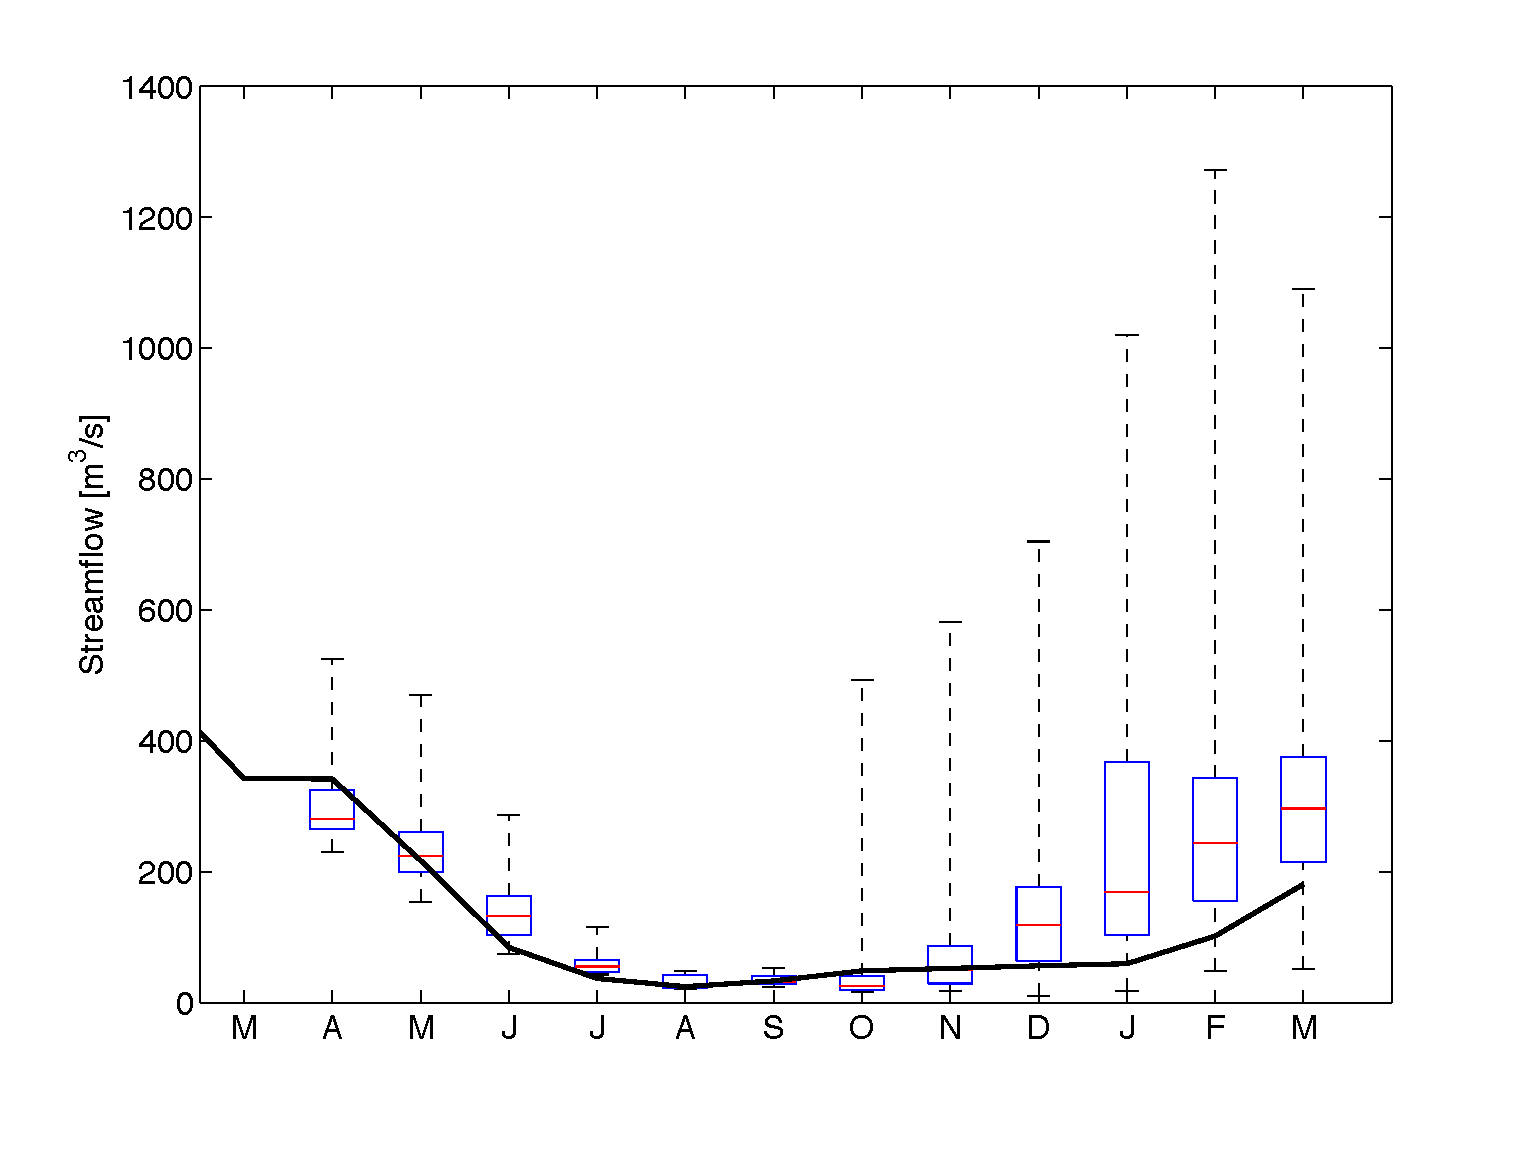
\includegraphics[width=\columnwidth]{Images/Introduction_Writing/boxplot_ensemble_2000.pdf} 
\caption[Streamflow forecast ensemble on April 1st 2000]{Streamflow forecast ensemble on April 1st 2000. The boxes show the 25\%, 50\%, and 75\% percentiles, while the whiskers represent the minimum and maximum ensemble members, thus indicating the full range of uncertainty. The solid black line represents the observations.}
\label{fig:boxplot_quality}
\end{figure}

Figures should always be good quality figures.
Axis tag, labels, and legend should have an appropriate font size.
Keep always the original figure (for example, \verb!.fig! if you created the figure with matlab): this will allow you or who is working with/after you to quickly modify it or recover the original data, if needed.
When applicable, keep the same axis ranges to the figures: it will ease the comparison between different figures.
When applicable/possible, use subfigures to ease the comparison between figures.

Finally, if you are using figures, tables and/or data from other sources, for example from other publications, cite always the reference. 
For example: \\
\blockquote{[...], taken/modified from Jones et al. (1950)}

\section{Mathematics}
Inline vs full line vs numbered equation.
Punctuation within equations.

Contemporary writers label the mathematical results in their papers as lemmas, theorems, propositions and so on.
Typically the major results of the paper are called theorems, the lesser results are called propositions.
The propositions are typically ingredients in the proofs of the theorems that are stand-alone statements of may be of independent interest), and the small technical results are called lemmas.
This probably varies quite a bit from writer to writer (and perhaps also from field to field).

\section{Margin notes}
Margin notes are used to study a new text or paper.
To read carefully a given text, it is essential that you write "all over" what you read, usually in the margins or between the lines?wherever there is space.
By annotating, you'll be creating a shorthand version of what you're reading to which you can return later for reference.
It's always much easier to navigate something you read a few days ago if you have taken detailed marginal notes.
We recommend to use margin notes when reviewing you own thesis.
Marginal notes help you to conceptualize the piece as you read.

Here are some general tips for annotating non-fiction articles.
Right next to each paragraph, write a brief phrase summarizing what happens in it. 
Underline passages that seem crucial to the point of the paragraph or to the larger thesis of the piece.
Note sections you don't fully understand with a question, like "What does this mean?" or "Doesn't this contradict my earlier argument?".
Outline points being made and the examples given to support them.
If you lists a number of reasons or factors that cause something or says something can be divided up into a certain number of parts, list the parts or factors in the margin.

\section{Submission to university: follow the instructions}
Visit \href{http://www.tedoc.polimi.it/tesilaurea/Consegna-tesi-di-laurea-(vecchio-ordinamento-e-specialistica)}{this link} for the updated information about the content of the thesis.

\enquote{Alcune Scuole forniscono linee guida specifiche cui i laureandi devono attenersi per la redazione della tesi. Per ulteriori informazioni:
\href{http://www.tedoc.polimi.it/download/lauree_magistrali/201406_POLITesi_Info_specifiche_scuole.pdf}{www.tedoc.polimi.it/\ldots}}

\subsection{Archiving electronic documents: PDF/A}
PDF/A is an ISO-standardized version of the Portable Document Format (PDF) specialized for the digital preservation of electronic documents. PDF/A differs from PDF by prohibiting features ill-suited to long-term archiving, such as font linking (as opposed to font embedding). The ISO requirements for PDF/A file viewers include color management guidelines, support for embedded fonts, and a user interface for reading embedded annotations.

Universities usually requires this standard but they're also not aware that common programs like MS Word, OpenOffice and so on aren't really able to produce compliant PDFs. In Latex, there's some development going on but at the time of writing, the available commands are still too obscure and buggy. So in the end, forget the PDF/A for now.\footnote{Or DIY and then make a pull request on github :D.}

	%\chapter{Practical guide to \enquote{ClassicThesis at DEIB}}
\label{chap:conclusion}
This template is ready to be used when writing a thesis at \myDepartment.
It is a modified version of Classic Thesis by Andr\'e Miede that can be found here \url{http://code.google.com/p/classicthesis/}.

\section{Learn \LaTeX}
\LaTeX\ is a document preparation system and document markup language.
It is widely used for the communication and publication of scientific documents in many fields, including mathematics, physics, computer science, statistics, economics, and political science.

\LaTeX\ users are weird people who care about the ligature between \enquote{f} and \enquote{i} and gets pissed off every time they look at a MS Word document.
Nevertheless, they can explain themselves very well as shown in some beautiful guides for the \LaTeX\ world.
Our preferred one for beginners is \enquote{The Not So Short Introduction to \LaTeXe}, which can be found \href{http://www.ctan.org/pkg/lshort}{here}.\footnote{\url{http://www.ctan.org/pkg/lshort}}
For italians we also strongly suggest \enquote{L'arte di scrivere con \LaTeX}, that can be found \href{http://www.lorenzopantieri.net/LaTeX_files/ArteLaTeX.pdf}{here}.\footnote{\url{http://www.lorenzopantieri.net/LaTeX_files/ArteLaTeX.pdf}}
It contains everything needed, however I suggest the reading of chapter 3 for a short introduction. \enquote{ClassicThesis} is another guide of the same author that can be useful, download it \href{http://www.lorenzopantieri.net/LaTeX_files/ClassicThesis.pdf}{here}.\footnote{\url{http://www.lorenzopantieri.net/LaTeX_files/ClassicThesis.pdf}}

\section{Install \LaTeX}
If you don't have already a \LaTeX\ system installed, this section will explain everything you need.
The easiest way to get \LaTeX\ is to install TeXLive, which works on all \acp{OS}.
In \url{https://www.tug.org/texlive/} you find the instructions and the files needed - and also get in touch with minimalism of \TeX users. 

Then you will need an editor: I strongly recommend TeXworks because it's very simple and available on all the platforms.
Also you don't need to install it, it's already included in TeXLive.
The official documentation of TeXworks is available \href{https://docs.google.com/file/d/0B5iVT8Q7W44pMk1WSFRKcDRlMU0/preview}{here};\footnote{\url{https://docs.google.com/file/d/0B5iVT8Q7W44pMk1WSFRKcDRlMU0/preview}}
I strongly recommend the reading of chapter 3.
Alternatevely you can read an italian manual: \href{http://profs.sci.univr.it/~gregorio/introtexworks.pdf}{profs.sci.univr.it/~gregorio/introtexworks.pdf} (just 13 pages, read it!).\footnote{If you already have a preferred editor, just keep using yours.}

After opening TeXworks, I strongly suggest to set these two additional things:
\begin{itemize}
	\item open Preferences, then go the Composition tab: in the second box there, the \enquote{Process instruments}, push the plus button.
	In the window just opened, write \verb!Biber! in the \enquote{Name} field, \verb!biber! in the \enquote{Program} field (lowercase!) and then press the plus button to add the argument \verb!$basename!;
	\item again in the same window, set \enquote{Hide console output} to \enquote{never}.
\end{itemize}

Then just test the installation of the template:
\begin{aenumerate}
	\item go into the template home folder;
	\item open the file \verb!ClassicThesis_DEIB.tex!;
	\item select \verb!pdfLaTeX! from the dropdown menu in the top right of the TeXworks window;
	\item press the rounded green button: it compiles the \verb!.tex! file for the first time and open the resulting \verb!.pdf!;
	\item select \verb!Biber! from the same dropdown menu and press again the green button: this compiles the bibliography, a thing you need to repeat only when you change the file \verb!Bibliography.bib!;
	\item select \verb!pdfLaTeX! again and recompile: this is needed to build indices and crossreferences;
\end{aenumerate}
The above compilation procedure is the standard way to translate the \LaTeX\ code into pdfs.

\subsection{Online editor}
If the above procedure seems too difficult to you and you have an internet connection always available, you might think to use an online editor.
The best choice at the time of writing is \url{http:\\\\sharelatex.com} where you can even find this template after registration to the site by looking for \enquote{Classic Thesis At DEIB}.
Your project will be saved on their server but you can also download them.
The platform allows up to two authors for free accounts.

There is no need to provide instructions for its use since the website has them.
They also have an online \LaTeX guide.

\section{Use \LaTeX\ within this template}

\subsection{File structure}
The template is organized in multiple file and folders:
\begin{aenumerate}

	\item \verb!ClassicThesis_DEIB.tex! is the main file to be compiled, found in the root folder.
	You should just add the source filenames you want to include and any hyphenation you need to explictly specify. 

	\item \verb!classicthesis-config.tex! contains options that can be chosen for this template, like the \verb!draft! one that prints date and time at the bottom of every page.
	It contains also the definition for the title, the author and others stuff displayed in the titlepage.
	Comments within the file should guide you.\footnote{comments are the rows starting with $\%$.} 
	Take a look at it!

	\item \verb!Bibliography.bib! is the \emph{Bibtex} database: it is a normal textfile where you should put books and articles read;

	\item \verb!Chapters! contains the files for the main chapters of your thesis; this is where you will add the chapters text, as well these very words in line 41 of the file \verb!Conclusion.tex!;

	\item \verb!CodeFiles! contains any code snippet you want to include in your thesis with the environment \verb!listings!; it might be some relevant Matlab or C code, as well as long bash scripts;

	\item \verb!FrontBackmatter! contains various files that are included in the main one to produce abstract, titlepages, acknowledgements, \ldots. 
	Follow the instructions below to modify them in order to suits your needs;

	\item \verb!Images! contains the \verb!.pdf! or \verb!.png! versions of the images of the thesis organized in subfolder per chapter.

\end{aenumerate}

To modify abstract, preface, acknowledgements snd acronyms, you need to go into the folder \verb!FrontBackmatter! where you will find the following:
\begin{description}

	\item[Abstract.tex] contains the text displayed as \enquote{abstract} and \enquote{sommario} just after the list of figures, tables, etc. Modify the text and leave the rest.

	\item[Acknowledgments.tex] contains the text put just before the table of contents. Modify the text to suit your needs.

	\item[Acronyms.tex] contains the environment \verb!acronym! with the definition of all the acronyms that will be used within the text. Add your own to the list and put the longest as parameter of the environment.
 
	\item[AutoParts] folder contains things that should work without your intervention. Forget them. 

	\item[Dedication.tex] same usage and structure as \verb!Acknowledgements.tex!.

	\item[Estratto.tex] Politecnico di Milano requires an italian long excerpt of theses written in foreign languages.

	\item[Frontespizio.tex] and \verb!FrontespizioIT.tex! are the cover page in english and italian, respectively. Politecnico di Milano requires the italian version of the english cover, so there it is. Both should work perfectly if you modify section 2 of the file \verb!classicthesis-config.tex!, but you may not like the style so modify them as you prefer.
	
	\item[Preface.tex] same usage and structure as \verb!Acknowledgements.tex!.

	\item[Publication.tex] same usage and structure as \verb!Acknowledgements.tex!, but not included by default. Activate it by uncommenting the relevant line in \verb!ClassicThesis_DEIB.tex!.

	\item[RetroFrontespizio.tex] contains the colophon. In most cases is fine as it already is.
\end{description}

\subsection{Special environments}\label{subsec:special_env}
In addition to common \LaTeX\ environments, this thesis is set to use:
\graffito{Use these environments: they make the thesis less bland and readable.}
\begin{itemize}
	\item the command \verb!\graffito{}! is used to create margin notes.
	The limits in number of words or length of word must be seen as a motivation to keep the notes short and simple;
	\item \verb!\begin{aenumerate}! to produce an \verb!\enumerate! with letters instead of numbers, as in the file list above;
	\item footnotes are useful to provide extra information. 
	Usually they are not required to understand a paragraph but provide interesting details. 
	This keeps the main body of text concise.
	You can create them with \verb!\footnote{text}!.\footnote{They should be placed after the punctuation mark and preferably at the end of the paragraph. In fact, they should not interrupt the reading flow. If you need to put a footnote in the middle of a paragraph, or of a sentence then the note should be part of the main text.}
	\item \verb!\ac{}! and its variations, defined by package \verb!acronyms!, provide nice handling for acronyms, like \ac{XML}, produced with the code \verb!\ac{XML}!.
	List them within the environment \verb!acronym! in the file \verb!FrontBackmatter/Acronyms.tex!.
\end{itemize}

\subsection{Citing, quoting and referencing}
References to bibliography are produced in the usual way with \verb!\cite{bib_key}! (\cite{bringhurst:2002}); don't forget the brackets which have to be added by hand.
There also variations of the command, like \verb!\citeauthor{bib_key}!, \verb!\citetitle{bib_key}! and others that you can find in the \verb!bibtex! manual.

\verb!\blockcquote[][]{}{}! \blockcquote[see][p. 111]{bringhurst:2002}{produce a quotation with reference to author and page}.
If the quotation is longer than two rows is indented.
This behavior is provided by the package \verb!csquotes!, which settings are in \verb!classicthesis-config.tex!. 
The package also provides \verb!\enquote{!the citation\verb!}! that produces \enquote{correct quotation style} according to the language in use.

There is a set of commands to refer to chapters, sections, subsections, appendices, figures, tables and equations, like \verb!\myChap{label_key}! to produce \myChap{chap:aChapter}.
There are also capital versions of the commands (\verb!\MyChap{}! produces \MyChap{chap:aChapter}).
They need a \verb!\label{name}! anchor next to the referred thing.
\begin{itemize}
	\item\verb!\myChap! for chapters;
	\item\verb!\mySec! for sections;
	\item\verb!\mySubsec! for subsections;
	\item\verb!\myAppendix! for appendices;
	\item\verb!\myFig! for figures;
	\item\verb!\myTab! for tables;
	\item\verb!\myEq! for equations;
\end{itemize}

\subsection{Figures and tables}
Figures are handled usually with the code
\begin{verbatim}
	\begin{figure}
	\centering
	\includegraphics[width=\columnwidth]{Images/your_image_name.pdf} 
	\caption[Short description]{Long description.}
	\label{fig:a_name}
	\end{figure}
\end{verbatim}
which produces things like \myFig{fig:massConstraintFeasibility}. 
Take care of the short description: it appears in the list of figures and should be just a reference, not a exhaustive description.
Of course, you need to put the image file \verb!your_image_name.pdf! in folder \verb!Images/!.
We suggest to keep things organized: create a folder for each chapter and keep the original source/working file in the same place.
	
\begin{figure}
\centering
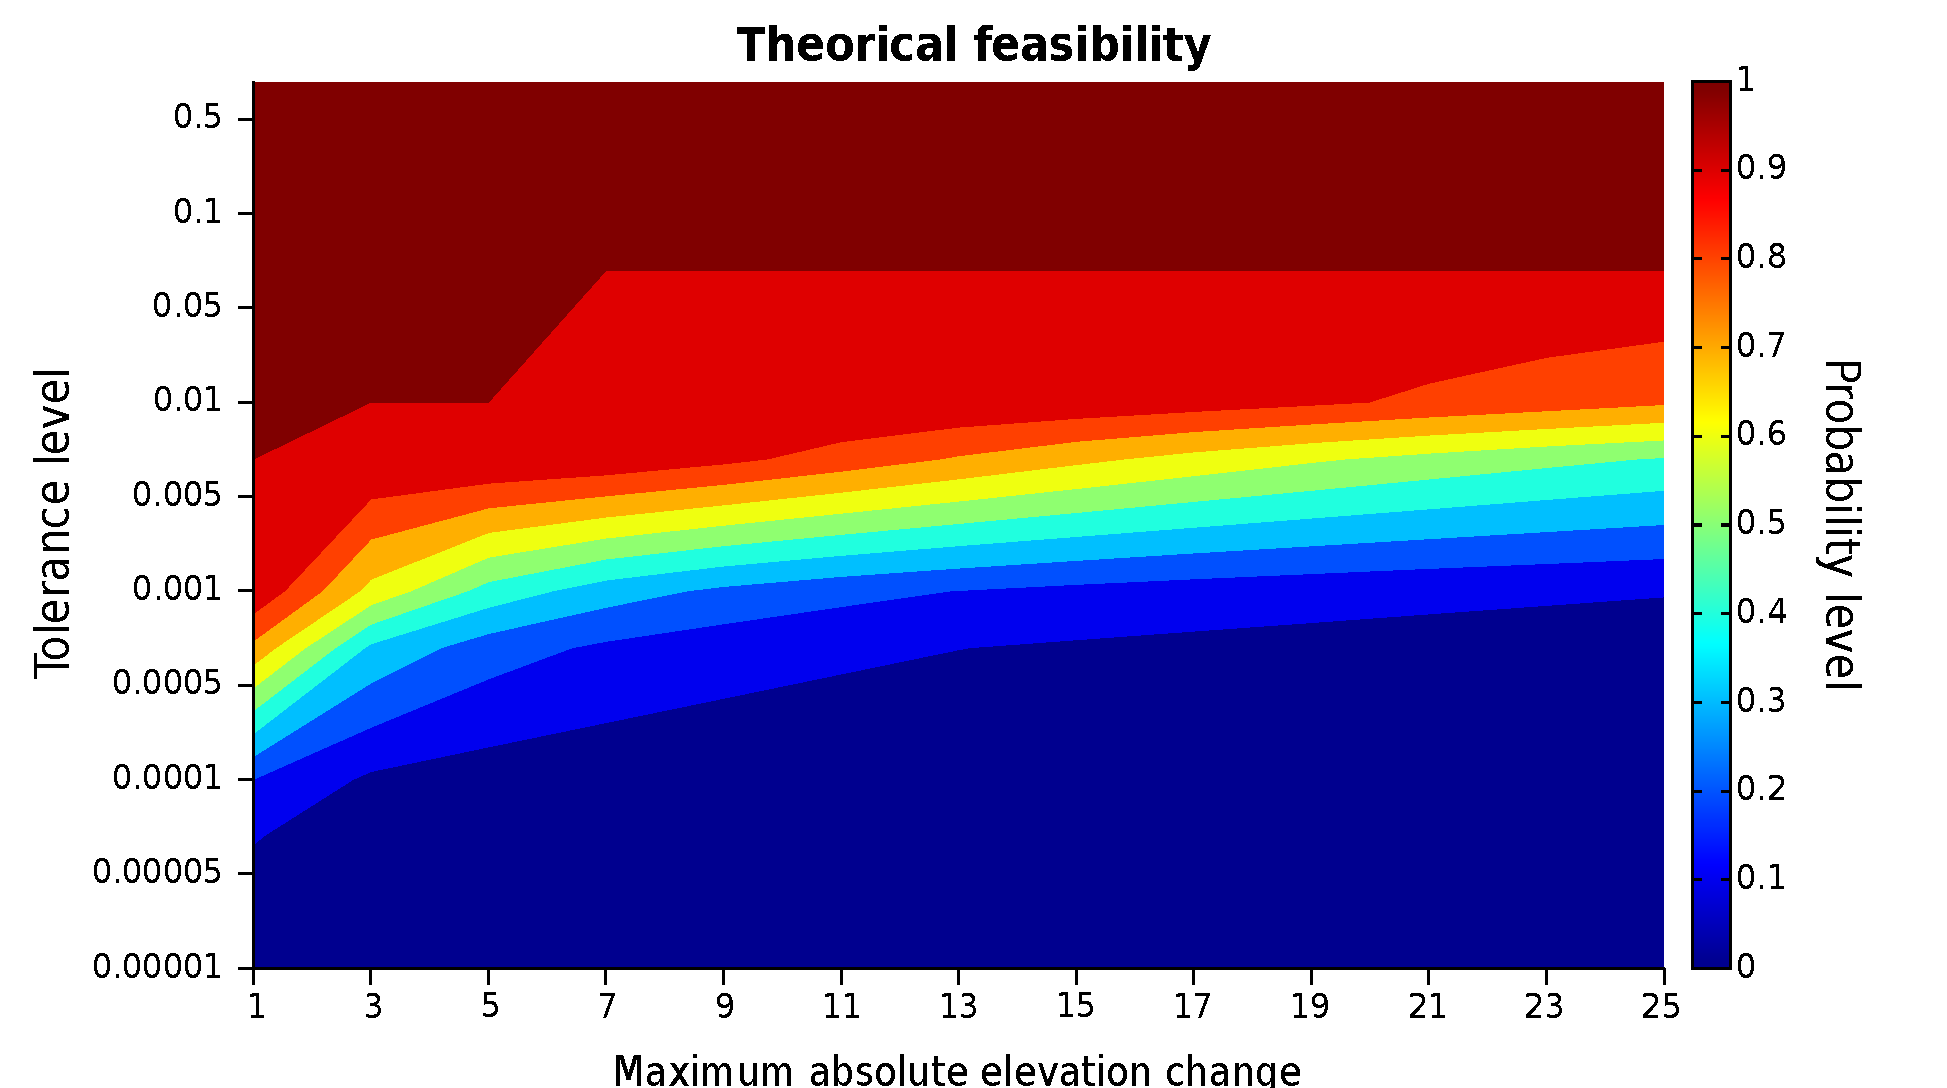
\includegraphics[width=\columnwidth]{Images/Technicalities/feasibilityNR51.pdf}  
\caption[Thing taken from our master thesis]{Thing taken from our master thesis whose meaning have been completely forgotten.}
\label{fig:massConstraintFeasibility}
\end{figure}

\begin{table}
\footnotesize
\centering
\begin{tabularx}{0.8\textwidth}{llrcl}
\toprule
\tableheadline{l}{Algorithm} &
\tableheadline{l}{Parameter} &
\tableheadlineMore{3}{c}{Suggested Values} \\
\midrule
\tablefirstcol{l}{Any}	& NFE	 		& $10\,000 $ 	& $ \div $ 	& $ 200\,000$ \\
				& Population Size 	&  $10 $ 		& $ \div $ 	& $ 1000$ \\
\midrule
\tablefirstcol{l}{GDE3} & DE step size 		& $0.0 $ 	& $\div $ 	& $ 1.0$ \\
				& Crossover rate 	& $0.0$ 	& $ \div $ 	& $ 1.0$ \\
\bottomrule
\end{tabularx}
\caption[Parameters needed for things]{Parameters needed for things that are not needed anymore themselves.}
\label{tab:MOEAandParameters}
\end{table}

Tables are produced with the code
\begin{verbatim}
	\begin{table}[tb]
	\footnotesize
	\centering
	\begin{tabularx}{0.8\textwidth}{llrcl}
	\toprule
	\tableheadline{l}{Algorithm} &
	\tableheadline{l}{Parameter} &
	\tableheadlineMore{3}{c}{Suggested Values} \\
	\midrule
	\tablefirstcol{l}{Any}
	& \acs{NFE} 		& $10\,000 $ & $ \div $ & $ 200\,000$ \\
	& Population Size 	&  $10 $ & $ \div 	$ & $ 1000$ \\
	\midrule
	\tablefirstcol{l}{\ac{GDE3}}
	& \ac{DE} step size & $0.0 $ & $\div $ & $ 1.0$ \\
	& Crossover rate 	& $0.0$ & $ \div $ & $ 1.0$ \\
	\bottomrule
	\end{tabularx}
	\caption[Short description]{Long description.}
	\label{tab:MOEAandParameters}
	\end{table}
\end{verbatim}
which produces \myTab{tab:MOEAandParameters}.
\verb!\myfloatalign!, \verb!\tableheadline{}{}! and its variation \verb!\tableheadlineMore{}{}{}! and \verb!\tablefirstcol{}{}! are used to give a common style to all tables in the document.
Use them!
They are defined in \verb!classicthesis-config.tex!.

\subsection{Math}
You can produce an equation like $\lim_{n \to \infty}\sum_{k=1}^n \frac{1}{k^2}= \frac{\pi^2}{6}$ by embedding this code in the line:
\begin{verbatim}
	$\lim_{n \to \infty}\sum_{k=1}^n \frac{1}{k^2}= \frac{\pi^2}{6}$.
\end{verbatim}

Equation that spans the full line like:
\[
\lim_{n \to \infty}\sum_{k=1}^n \frac{1}{k^2}= \frac{\pi^2}{6}
\]
are produced with something like this:
\begin{verbatim}
	\[
	\lim_{n \to \infty}\sum_{k=1}^n \frac{1}{k^2}= \frac{\pi^2}{6}.
	\]
\end{verbatim}
If you need to refer to the equation later on, you need to number and label it. It is done via
\begin{verbatim}
	\begin{equation}
	\label{eq:euler}
	e^{i\pi}+1=0.
	\end{equation}
\end{verbatim}
\begin{equation}
	\label{eq:euler}
	e^{i\pi}+1=0.
\end{equation}
From \myEq{eq:euler} you can see how \verb!\myEq{eq:euler}! should be used.

Numeric sets requires specific font as $\forall x \in \mathbb{R}$ which is produced with \verb!$\forall x \in \mathbb{R}$!. Matrices like
\[
A=
\begin{bmatrix}
x_{11} & x_{12} & \dots \\
x_{21} & x_{22} & \dots \\
\vdots & \vdots & \ddots
\end{bmatrix}
\]
requires
\begin{verbatim}
	A=
	\begin{bmatrix}
		x_{11} & x_{12} & \dots \\
		x_{21} & x_{22} & \dots \\
		\vdots & \vdots & \ddots
	\end{bmatrix}.
\end{verbatim}
Multiline equation can be produced with different environments like \verb!split! and \verb!cases!.
\[ 
\begin{split} 
a &= b+c-d \\ 
  &= e-f \\ 
  &= g+h \\ 
  &= i. 
\end{split} 
\]
comes from
\begin{verbatim}
	\begin{split} 
	a &= b+c-d \\ 
 	&= e-f \\ 
	&= g+h \\ 
	&= i. 
	\end{split}. 
\end{verbatim}
\[
f(n):=
\begin{cases} 
2n+1, & \text{con $n$ dispari,} \\ 
n/2,  & \text{con $n$ pari.} 
\end{cases} 
\]
comes from
\begin{verbatim}
	\begin{split} 
	a &= b+c-d \\ 
 	&= e-f \\ 
	&= g+h \\ 
	&= i. 
	\end{split}. 
\end{verbatim}

Definition like
\begin{definition}[Gauss] 
The math guy find obvious that
$\int_{-\infty}^{+\infty}
e^{-x^2}\,dx=\sqrt{\pi}$. 
\end{definition}
are produced with the code 
\begin{verbatim}
\begin{definition}[Gauss] 
The math guy find obvious that
$\int_{-\infty}^{+\infty}
e^{-x^2}\,dx=\sqrt{\pi}$. 
\end{definition}
\end{verbatim}
There also a number of other similar environments, like \verb!observation!, \verb!theorem! with or without name, \verb!corollary! and \verb!lemma!.
\begin{observation}
But many people like me don't find it obvious.
\end{observation}
\begin{theorem} 
Mathematicians are very rare, if any.
\end{theorem} 
\begin{theorem}[Pythagorean]
The square of the hypotenuse of a triangle is equal to the sum of the squares of the other two sides.
\end{theorem}
Demonstration is left for exercise.
\begin{corollary}
A line segment whose length is incommensurable so the ratio of which is not a rational number, can be constructed using a straightedge and compass. 
\end{corollary}
\begin{lemma}
Pythagoras's theorem enables construction of incommensurable lengths because the hypotenuse of a triangle is related to the sides by the square root operation.
\end{lemma}
You can also proof your theorem with the environment \verb!proof!.
\begin{theorem}[Surprise]
We have $\log(-1)^2=2\log(-1)$.
\end{theorem} 
\begin{proof} 
We have $\log(1)^2 = 2\log(1)$.
But also we have $\log(-1)^2=\log(1)=0$.
So $2\log(-1)=0$.
\end{proof}
There's also the cute little square at the end.

\section{Contributing to this template}
Suggestion and improvements are welcome at \url{https://github.com/Lordmzn/ClassicThesis-at-DEIB} or via email at \url{emanuele.mason@polimi.it}, \url{andrea.cominola@polimi.it} or \url{daniela.anghileri@polimi.it}. 
	\chapter{Introduction} \label{chap:intro}

\begin{flushright}{\slshape    
Electrical science, too, by its fascination, by its promises of immense realizations, of wonderful possibilities chiefly in humanitarian respects, has attracted the attention and enlisted the energies of the artist; for where is there a field in which his God-given powers would be of a greater benefit to his fellow-men than this unexplored, almost virgin, region, where, like in a silent forest, a thousand voices respond to every call?}
   \\ \medskip --- \citeauthor{on_electricity:1897}
   \citetitle{on_electricity:1897} \citeyear{on_electricity:1897}
\end{flushright} 

The electric motors made their first appearances in the middle of the XIX century right after the invention of the battery by the Italian physicist, chemist and inventor Alessandro Volta in 1800, the discovery of the generation of a magnetic field from an electric current by the Danish physicist and chemist Hans Christian \O rsted in 1820 and the invention of the electromagnet by the English physicist William Sturgeon in 1825 (\citeauthor{ETI_motorHistory}, \citeyear{ETI_motorHistory}). After these foundations were laid, the development of a machine that generates mechanical power from electrical power has been improving day by day, and, along with that improvement, also its utility has been increasing.

\begin{figure}[htbp]
\centering
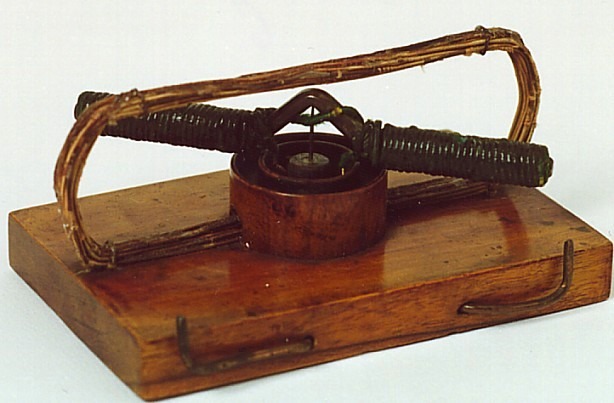
\includegraphics[width=\columnwidth]{Images/jedlik_motor.png} 
\caption[Jedlik's "Electromagnetic Self-Rotor"]{Jedlik's "Electromagnetic Self-Rotor". The historic motor created by the Hungarian physicist \'Anyos Jedlik still works perfectly today in the Museum of Applied Arts in Budapest.}
\label{fig:jedlik_motor}
\end{figure}

Due to the reduction of the prices of metals and the improvement and automation of manufacture processes, electric motors became available for a large range of applications, and not only as a research topic, up to the point that nowadays we interact with them in our daily life, sometimes without even noticing it. We have electric motors in all types of devices, from small applications like home appliances and hand-held gadgets, to large applications like robotics, cars and spaceships. As the complexity of the application increases, also the need for accuracy and efficiency does, leading to the development of more advanced electric motor technologies which lead to complex motion control techniques.

One of the most complex applications for motor control is robotics. The motion in a robotic system is part of its definition of automatic movement, therefore, a robotic system needs a predictable driving system to fulfil its purpose, which implies that most of the parameters of the motors inside the robot are known and that they can be controlled in a correct and precise way.

A challenging application regarding motors in robotics is the wheel driving, since it needs to be precise and powerful at the same time to transport the robotic system around large surfaces in an unmanned way, which means that there is no person on board and controlling the robot. For example, in robotic agriculture, which is one of the main reasons why this work was developed, a robot becomes an unmanned vehicle, which must transport itself around in farms, where the road represents harsh conditions for transportation, introducing the need for a precise drive to deal with small crops, a high torque to transport the robot in uneven grounds and a good range of speeds to displace itself in large field areas in the fastest way possible.

With aims to propose a solution for the land transportation in robotic agriculture projects, different types of motor technologies were studied a priori, finding out that in-wheel permanent-magnet brushless motors are one of the most suitable and currently used solutions to develop electric vehicles, since they don’t need an external system for power transmission from the motor to the wheels, taking advantage of the high stall torque property of the electric motors and the reduction of the space and weight that having a motor inside a wheel represents (\citeauthor{robi:2017}, \citeyear{robi:2017}).

To correctly drive permanent-magnet brushless motors, it is necessary to apply a proper driving technique, which becomes a complex task when the goal is to achieve the desired characteristics mentioned previously: a good precision, a high torque and a large range of speed. Given such a challenge, the development of electric motor drives becomes one of the topics that draws the interest of many engineers and scientists, also due to the multidisciplinary approach needed to reach the speed, torque and efficiency required to drive the development that the inventions of tomorrow require. The approach to improve the motor drive in the electronics engineering field is directly related to the development of the driving circuit topology and to the implementation of complex control algorithms in embedded software that improve the performance of the different motor technologies available.

Since the brushless motor technology is quite recent in comparison with the rest, there is still a lot of development going on regarding its driving, with aims to reach the highest efficiency possible at the lowest cost. The objective of this work was to develop an electronic driver to control brushless motors, taking as a study case the in-wheel motors that transport a skid-steering robot designed for robotic agriculture. We studied the available electronic architectures to design a motor driver, the different approaches to drive brushless motors, like the trapezoidal and the sinusoidal drive and the peripherals needed to make these driving happen. After studying these topics, the motor driver was physically implemented and tested, and from this, a new architecture was proposed from the results and conclusions obtained from the implementation and testing of the circuit.

\begin{figure}[htbp]
\centering
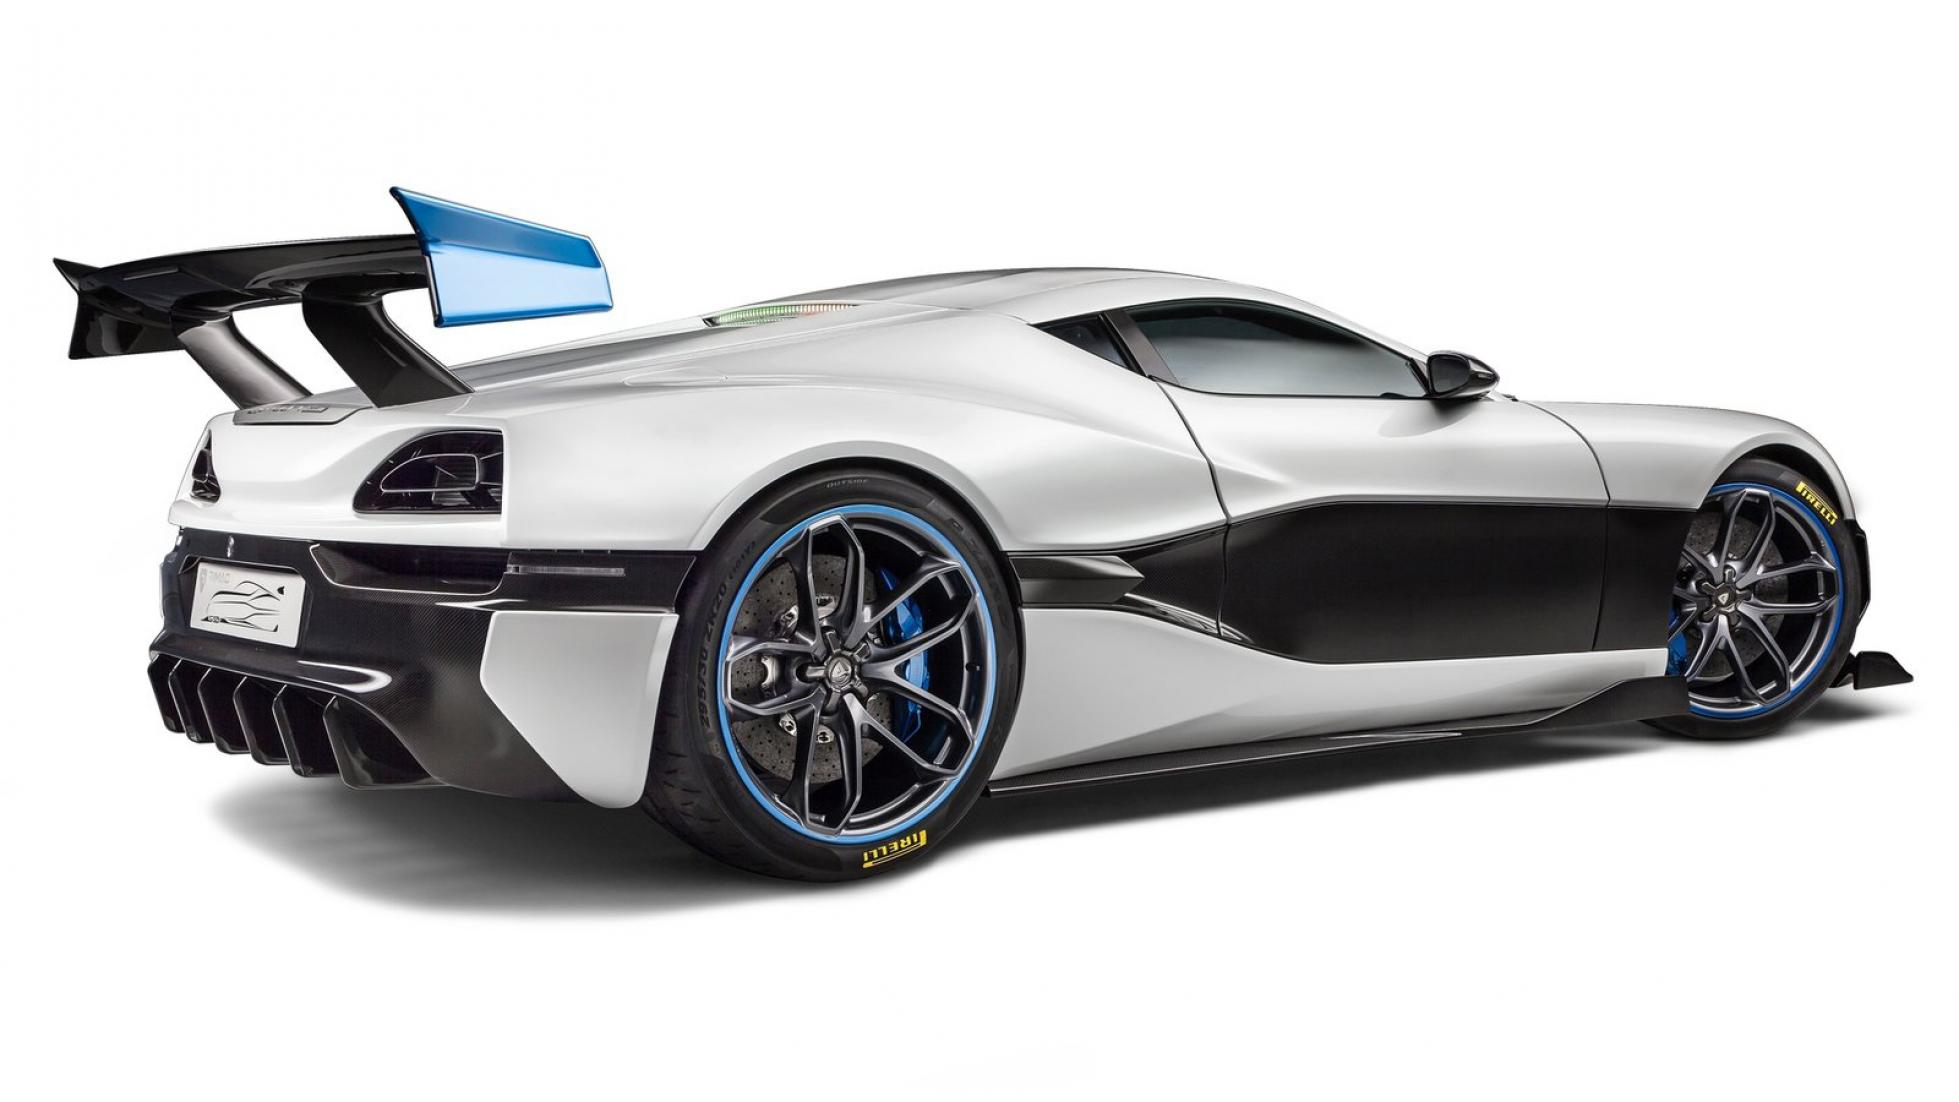
\includegraphics[width=\columnwidth]{Images/rimac-concept_s4.png} 
\caption[Rimac Concept S]{Rimac Automobili's electric supercar Concept S. Electric cars are becoming a trend and one of the main drivers for the development of technology related to electric motors.}
\label{fig:rimac_concept_s}
\end{figure}

This thesis explains in detail the most important information regarding the physical implementation of a motor driving system in such a way that it can be fully replicated. In Chapter \ref{chap:problem}, we explain more in detail the different reasons why this work was developed and the focus points that were stressed out. In Chapter \ref{chap:theory}, a simple but sufficient explanation about the theory behind the electric motor is given, explaining also the different existing technologies and their particular driving methods. In Chapter \ref{chap:robi} we explain the study case of ROBI', a prototype mobile manipulator for agricultural applications, which uses the in-wheel motor for which the motor driver of this work was developed. In Chapter \ref{chap:implementation} we explain in deep detail all the work developed around the implementation of the motor driver, both in the software and the hardware fields. In Chapter \ref{chap:results} we explain the final results of the work, showing and comparing graphs and waveforms of the behaviour of the in-wheel motor driven by the system developed. Finally, on Chapter \ref{chap:conclusion}, we discuss the results of the work realized and propose a new system, based on the implementation of the researched architecture and the problems encountered while working on the project. 
	\chapter{Problem Statement} \label{chap:problem}

As motion applications complexity increases, like in the robotics field, the need for a more complex and robust driving system arises, and with it, the need to make decisions regarding the technologies to be implemented for them. For example, when a robotics project begins, with the objective to implement a solution that hasn't been implemented before, one of the main concerns is the motion system. The selection of the motor that is going to be used in a project is not an easy task, since many details must be considered, like the speed and torque required by the application, which lead to the selection of the motor technology, which might be limited by the available power source, the computing power and the economic budget of the project. These aspects have a strong dependency between each other and choosing each one of them represents a trade-off that must be studied in detail to reach an optimal result for the desired application.

\section{Technological Trade-Offs}\label{sec:research_questions}

One of the main goals in the technology research and development has always been to reduce the trade-offs between the most important parameters in different engineering applications, using the most suitable technologies available, depending on the application requirements. One of the fields of engineering that has a big focus on the reduction of trade-offs is the motor drive research, since their development is crucial to drive innovation in many engineering fields.

A complicated trade-off to deal with is the cost of a motor drive, which is one of the most limiting characteristics project developments, both for research activities and for industrial and consumer applications. If a project is not expected to generate an income after its development or it’s not backed up by a research institute with resources, or if the product is expected to be kept at a low price for many different reasons (like accessibility for low income communities or the possibility of large expansion), the price of a motor drive might be the weak side in a trade-off analysis and the development of the project might not be optimal, since it might require more work to reach an acceptable result.

\section{Learning Curve}\label{sec:objectives}

The cost of a project leads to another important trade-off on engineering research and development: the learning curve. In some areas like robotics, a professional engineering project requires thousands of hours of man-work to reach a desirable result. An important amount of the time available for these projects is used in learning theory regarding the technology related to the project and how the available tools for such technology work. This time consumed in learning all the information needed regarding a project is called “learning curve”. The amount of work necessary to reach a good result makes most of the engineering projects expensive and, in many cases, a big part of that time is consumed by the learning curve, time that could be used for developing another part of the project, increasing the speed of the development and, therefore, reducing its cost.

\section{Motor Driver Development}\label{sec:methods}

With the aim to solve these two important trade-off factors in motor driving systems, we decided to study the possibility to reduce the cost of a motor drive by using a driver based on a cheap architecture which can be easily modified and allows to understand in a fast way how the motor driver works, making the development around it faster and easier for future projects.

To set up the design specifications for the motor driver to be studied, we based the requirements in the drive characteristics of a robot designed for robotic agriculture designed by the engineering group of the AIRLab of the Politecnico di Milano called ROBI' (\citeauthor{robi:2017}, \citeyear{robi:2017}). This robot is driven by four in-wheel brushless motors that will be described in detail in Chapter \ref{chap:robi}.\\

\section{Implementation of Field Oriented Control}\label{sec:novelties}

Having the objective defined, we looked for an already available platform to develop a motor driver with aims to look for points to improve and define a platform that could be used for different projects involving \acf{PMAC} motors, both \acf{BLDC} and \ac{PMSM}. With this aim, we found a board called VESC Board, developed by the Swedish engineer Benjamin Vedder, who made available all the files for its production, including the schematic circuits, the bill of materials, the \acf{PCB} layout files and the source code. Vedder’s circuit was very appealing since it had many ports available and it was based on a technology that is easy to study since it’s based in a design proposed by Texas Instrument for three-phase motors.

Since this motor driver was needed to be used in robotics applications, we had the necessity to modify the source code of the microcontroller to apply motor control methods that would be different to the ones available for the VESC board since the code available was designed to drive an electric skateboard. For this aim, we decided to develop our own source code, this way we would have control over everything developed by us and the expansion of the code would follow up without the need of doing reverse engineering over the code that was already available.

Since the motors of the wheels of the robot are \ac{PMSM}, they have a sinusoidal configuration, and therefore, a sinusoidal waveform was needed to be applied into the motor to reach an optimal efficiency and to control the speed even in low speeds. This specification pointed us towards the implementation of the \acf{FOC} method, which improves the torque capabilities of the motor at controlled low speeds as it will be explained in Chapter \ref{chap:theory}. 
	\chapter{Motor Control Theory} \label{chap:theory}

In this chapter, we will review some theoretical principles that concern us regarding motor control. First, we will review the physical principles that rule over the electric motors and we will explain the different motor technologies and its configurations, focusing in the \acf{PMAC} motors. Later, we will review the motor drives, the configuration of a driver and the different driving techniques for the \ac{PMAC} motors. Finally, we will explain the control methods that can be applied to them.

Most of the theory in this chapter was taken from the book \citetitle{sistemi_di_controllo:2007}, by \citeauthor{sistemi_di_controllo:2007}, \citeyear{sistemi_di_controllo:2007} and from the compilation \citetitle{AC_drives}, by \citeauthor{AC_drives}, \citeyear{AC_drives}.


\section{Electric Motor}

An electric motor is an electric machine that transforms electrical power (product between voltage and current):

\begin{equation}
	\label{eq:e_elec}
	P_{electrical} = V \cdot I
\end{equation}

into mechanical power (product between torque and angular speed):

\begin{equation}
	\label{eq:e_mech}
	P_{mechanical} = T \cdot \omega
\end{equation}

by means of the electromagnetic phenomena that takes place inside the motor, which is explained by the physical principles mentioned in this chapter.

\subsection{Physical Principles} \label{physical_principles}

The generation of torque in electric motors is based in the interaction of two magnetic fields, one generated by magnets or windings placed in the stator and the other one generated by magnets or windings placed in the rotor as seen in Figure \ref{fig:motor_assembly}.

\begin{figure}[htbp]
\centering
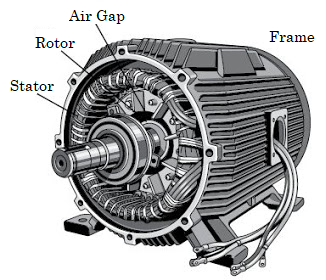
\includegraphics[width=8cm]{Images/motor_assembly.png} 
\caption[Partially Assembled Motor]{Partially Assembled Motor. An electric motor consists mainly in three parts: a rotor, which moves due to the electromagnetic interaction; a stator, the body of the motor; and a frame, which holds the rotor and the stator together. The air gap is the space betweeen the rotor and the stator, where the electromagnetic interaction takes place (\citetitle{basic_components}, \citeyear{basic_components}).}
\label{fig:motor_assembly}
\end{figure}

The physical laws that rule over the electric motor are mainly four: The Lorentz’s Law, which helps us define the torque generated by an electric charge moving inside a magnetic field; Faraday’s Law of Electromagnetic Inductance and the Lenz’s Law, which explain the generation of the \acf{BEMF} in the motor coils depending on the speed of the rotor and the influence of the magnetic field generated due to this BEMF respectively; and the Ampere-Laplace Law, which allows us to calculate the magnetic field of a current loop and the mechanical interaction between two magnetic fields.

\begin{description}

\item[Lorentz's Law] defines a force $F$, which acts over an electric charge $q$ moving with a speed $v$ inside a magnetic field with intensity $B$ as seen in Figure \ref{fig:lorentz_law}:

\begin{equation}
	\label{eq:force_1}
	F = q v \times B
\end{equation}

By defining a current $I$ passing through a conductor with length $l$ we can transform Equation \ref{eq:force_1} into Equation \ref{eq:force_2}:

\begin{equation}
	\label{eq:force_2}
	F = l I \times B
\end{equation}

Considering the current $I$ flowing through a conductive loop as the one in Figure \ref{fig:lorentz_law} with sides lengths $l$ and $h$ we can see that there is a force $F$ generated in the direction of the cross product of the current $I$ and the magnetic field $B$. The maximum force $F$ is generated in the sides of the loop where the direction of the current $I$ is perpendicular to the direction of the magnetic field $B$ ($ab$ and $cd$), while on the other two sides ($ad$ and $bc$) the forces generated are cancelled with each other due to the direction of the current respect to the magnetic field.

\begin{figure}[htbp]
\centering
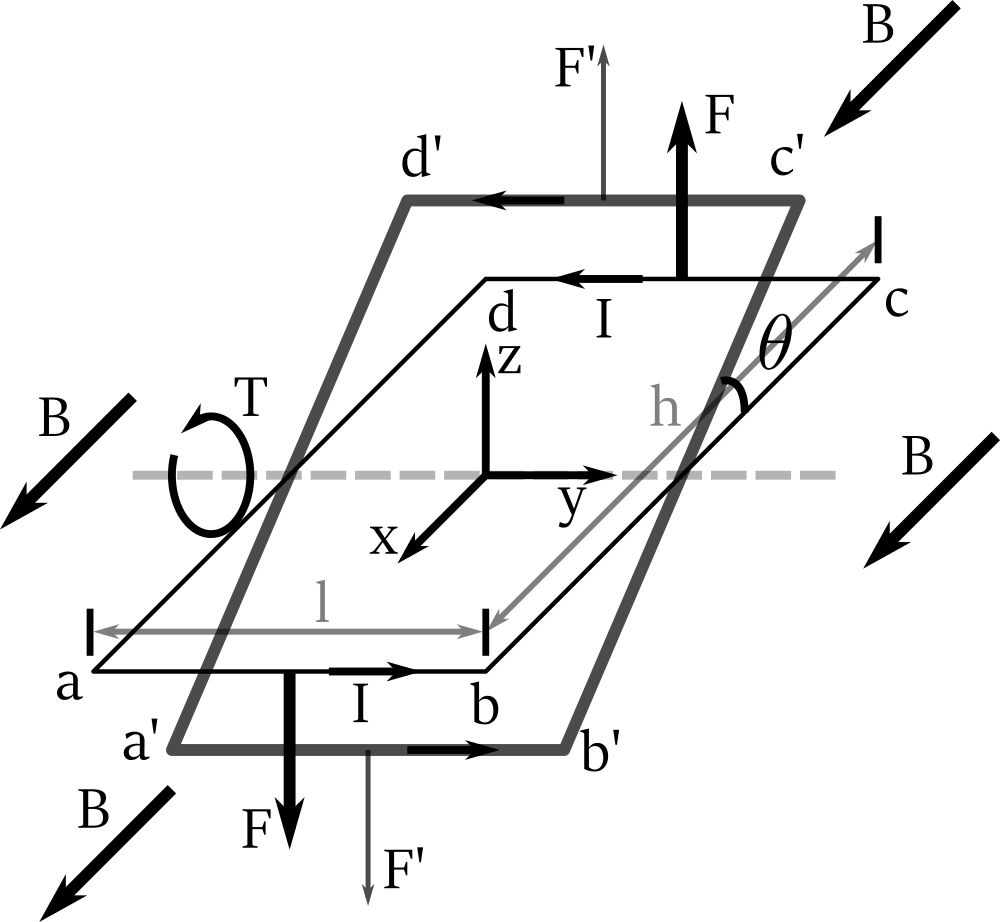
\includegraphics[width=8cm]{Images/lorentz_law.png} 
\caption[Lorentz's Law Diagram]{Visual explanation of the interaction of the current $I$ and the magnetic field $B$ generating a force $F$ and, consecuently, a torque $T$ around the $y$ axis (\citeauthor{sistemi_di_controllo:2007}, \citeyear{sistemi_di_controllo:2007}).}
\label{fig:lorentz_law}
\end{figure}

Since the forces $F$ generated on the sides $ab$ and $cd$ have the same magnitude but different direction, they create a torque $T$ around the $y$ axis defined by the magnetic field, the current and by the length of the sides of the loop as:

\begin{equation}
	\label{eq:torque_1}
	T = I h l B \cos \theta
\end{equation}

We can see in Figure \ref{fig:lorentz_law} and in Equation \ref{eq:torque_1} that when the angle $\theta$ between the sides $ad$ or $bc$ and the direction of the magnetic field $B$ is $\pi / 2$ radians, the torque $T$ is zero and when the angle $\theta$ is zero or $\pi$ radians, the torque reaches its maximum possible value. 

The dependency of the torque created by the interaction of the current and the magnetic field on the angle between these two physical quantities introduces the need of changing the direction of the magnetic field or the direction of the current, hence, the polarity of the loop, to maintain the loop spinning and a non-zero torque.

\item[Faraday’s Law of Electromagnetic Induction] states that
\blockquote{In every circuit under the effect of a magnetic field, an electromotive force is induced equal to the derivative respect to the time of the magnetic flux passing though the circuit, with negative sign. (\citeauthor{emWaves:1968}, \citeyear{emWaves:1968})}

therefore, by indicating with $E$ the electromotive force and with $\phi _{m}$ the magnetic flux, we have:

\begin{equation}
	\label{eq:em_1}
	E = - \frac{\mathrm{d} \phi _{m}}{\mathrm{d} t}
\end{equation}

If we consider a case like the one in Figure \ref{fig:lorentz_law} we can calculate the magnetic flux passing though the loop as:

\begin{equation}
	\label{eq:mf_1}
	\phi _{m} = B \cdot u_{N} S = B \cdot u_{N} h l = h l B \sin \theta 
\end{equation}

where $S$ is the surface of the loop and $u_{n}$ is the direction normal to the plane of the loop. Therefore, we get an induced electromotive force of:

\begin{equation}
	\label{eq:em_2}
	E = - \omega h l B \cos \theta
\end{equation}

where $\omega$ is the angular speed of the loop. We can see, comparing Equation \ref{eq:em_2} and Equation \ref{eq:torque_1}, that the induced electromotive force depends on the angular speed in the same way than the acting torque depends on the current.

\item[Lenz's Law] can be explained after the explanation of the induced electromotive force. It states that the induced current in a loop has the direction that creates a magnetic field that opposes the change in magnetic flux through the area enclosed by the loop, therefore, the induced current tends to keep the magnetic flux $\phi _{m}$ from changing in the circuit.

If the rotation of the loop is generated by the circulation of a current inside a magnetic field, the induced electromotive force will try to oppose to the pass of the current, that’s why it’s normally referred to as \acf{BEMF}.

\item[Ampere-Laplace Law] is the last piece to understand the transformation of electrical energy into mechanical energy. It allows us to calculate the magnetic field generated by a closed loop conducting current in a point defined by a vector $p$ as:

\begin{equation}
	\label{eq:B_1}
	B(p) = \frac{\mu_{0}}{4 \pi} \oint I \frac{u_{t} \times u_{r}}{r^{2}}dl
\end{equation}

where $\mu_{0}$ is the vacuum magnetic permeability constant, $I$ is the current circulating through the loop, $u_{t}$ is the versor with direction of the current in the infinitesimal element $dl$ and $u_{r}$ and $r$ are versor and module that define the point $p$ respect to the infinitesimal element of the loop.

Given that the magnetic fields can be generated both by permanent magnets and by current circulation, the electromechanical conversion is obtained due to the interaction of two magnetic fields according to the alignment principle:

\blockquote{In a region of space which hosts two magnetic fields, there is a mechanical action that tends to align both fields. (\citeauthor{sistemi_di_controllo:2007}, \citeyear{sistemi_di_controllo:2007})}

So, if we consider the loop from Figure \ref{fig:lorentz_law} and Equation \ref{eq:B_1}, we can see that there is a magnetic field generated around the loop as seen in Figure \ref{fig:alignment}, and due to the alignment principle, we will get the strongest coupling torque when the magnetic fields are perpendicular to each other.

\begin{figure}[htbp]
\centering
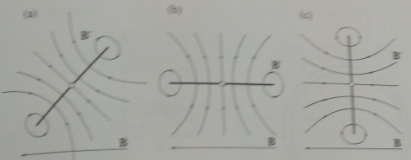
\includegraphics[width=8cm]{Images/alignment.png} 
\caption[Alignment Principle]{Visual explanation of the alignment principle. The alignment torque is the largest in the configuration of figure B and nule in the configuration of figure C.}
\label{fig:alignment}
\end{figure}

In the case of electrical motors, there are two different magnetic fields generated in the airgap due to the permanent magnets or to the windings placed in the stator and the rotor which can be considered in radial direction, described by two magnetic fields $B_{r}(\theta,t)$ and $B_{s}(\theta,t)$, from which interaction we get the electromechanical conversion, since we have the generation of a torque which tends to align the two fields angles where they have the largest intensity. The alignment torque will be an expression of the type:

\begin{equation}
	\label{eq:torque_2}
	\tau_{m} = k B_{r} B_{s} \sin \delta
\end{equation}

where $\delta$ is the de-phasing angle between the two fields and the maximum torque will be when $\delta = \pi / 2$.

\end{description}

In conclusion, by feeding the windings in the right way, we look forward to having a constant 90° de-phase between the two magnetic fields in aims to obtain the maximum torque generation.

In the case of the \acf{DC} motor, the perpendicularity condition is maintained by a polarity commutating structure attached to the rotor which is connected to the windings that generate the rotor magnetic field that tries to align itself to the magnetic field of the permanent magnets attached to the stator. This commutating system is connected to the power supply by metallic brushes that energyse the motor until it reaches a certain angular position and the commutating lead changes to the next one, changing the polarity of the windings. Therefore, the torque obtained is independent from the position of the rotor and it’s proportional to the amplitude of the power source.

\begin{figure}[htbp]
\centering
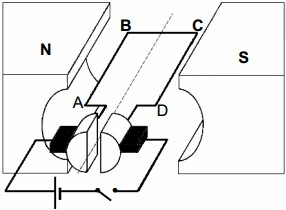
\includegraphics[width=8cm]{Images/dc_motor.png} 
\caption[DC Motor Scheme]{Basic schematic representation of the \ac{DC} motor using the same loop represented in Figure \ref{fig:lorentz_law}}
\label{fig:dc_motor}
\end{figure}

Brushless motors, which will be explained later in this chapter, the perpendicularity condition is maintained by feeding in the right time the windings in function of the angular position of the rotor $\theta$, which is one of the main goals to be achieved and explained in this work.

\section{PMAC Motors}

The \acf{PMAC} motor is a kind of electrical motor that doesn't need the mechanical commutators mentioned in \ref{physical_principles} to be driven as in the case of the DC motor, but its windings need to be energysed in a specific way to function correctly. Since it doesn't need the mechanical commutators, it also doesn't need the brushes that energyse the windings, so it can be said that it's a brushless motor. As seen in Figure \ref{fig:brushless_section}, there are permanent magnets attached to its rotor and the coils are winded into its stator in a three-phase configuration.

\begin{figure}[htbp]
	\centering
	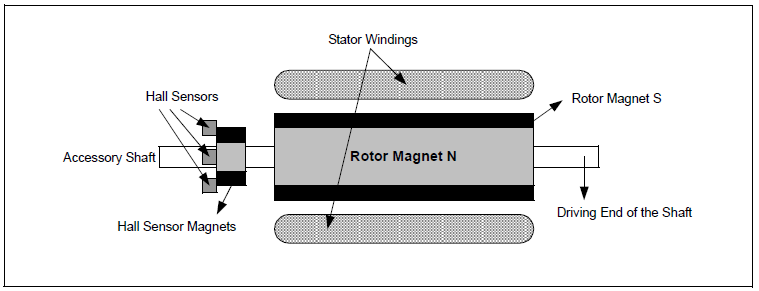
\includegraphics[width=12cm]{Images/brushless_section.png} 
	\caption[Brushless Motor Transverse Section]{Brushless motor transverse section (\citeauthor{microchip}, \citeyear{microchip}).}
	\label{fig:brushless_section}
\end{figure}

These three phases are fed alternativelly in such a way that the magnetic field, generated by the relative currents passing through the coils, should always be orthogonal and synchronous to the magnetic field generated by the rotor's permanent magnets. The characteristics mentioned above give the name to this kind of motors. 

To maintain the synchronization, it's necessary to commute, by means of an inverter as the one represented in Figure \ref{fig:inverter_1}, the currents in the windings of the stator, taking as a reference the angular position of the rotor, which must be obtained by a sensor.

The number of commutations needed to generate one revolution of the rotor is determined by the number of times that each phase coil is winded in the stator. For example, if each phase coil of the three phase system is winded only once, one commutation would be enough to generate one revolution, but if each phase coil is winded 6 times, we would need to commutate the power supply of the coils six times to generate one revolution. This ratio is called \acf{PP}. Normally, the \ac{PMAC} motors have many \ac{PP} (six or more) in order to have a lower torque ripple since the alignment of the magnetic fields would be every $360\degree/(\ac{PP} \times \Phi_{N})$ degrees of the rotor. For the study on the electromechanical conversion, the angular position of the rotor is substituted by an electrical angular position, which is controlled by the commutator and is defined by:

\begin{equation}
	\label{eq:pole_pairs}
	\theta_{electrical} = \ac{PP} \theta_{mechanical}
\end{equation}

which also represents a relationship between the mechanical speed of the rotor and the electrical speed of commutation, which is defined by the commutation frequency:

\begin{equation}
	\label{eq:pole_pairs}
	\omega_{electrical} = f_{commutation} = \ac{PP} \omega_{mechanical}
\end{equation}

so, for example, if we have a motor with 6 \ac{PP} and we want to drive it at $1 kHz$, we must commutate the polarity of the inverter at $f_{commutation} = \ac{PP} \omega_{mechanical} = (6) (1 kHz) = 6 kHz$.

\begin{figure}[htbp]
	\centering
    \subfloat[2 Pole Pairs\label{subfig-1:2_pole}]{%
    	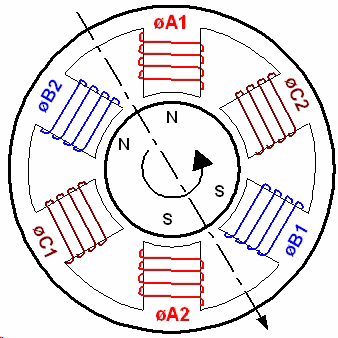
\includegraphics[width=0.3\textwidth]{Images/2_pole.png}
    }
    \hfill
    \subfloat[2 Pole Pairs\label{subfig-2:4_pole}]{%
      	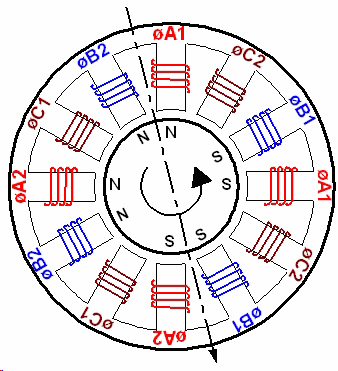
\includegraphics[width=0.3\textwidth]{Images/4_pole.png}
    }
    \hfill
    \subfloat[2 Pole Pairs\label{subfig-3:6_pole}]{%
      	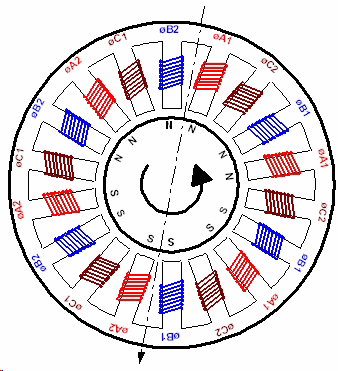
\includegraphics[width=0.3\textwidth]{Images/6_pole.png}
    }
    \caption{Different pole pair configurations}
    \label{fig:pole_pairs}
    %https://www.basilnetworks.com/article/motors/brushlessmotors.html
\end{figure}

The main characteristics that make the brushless motor a better option for some applications than the \ac{DC} motor are the following:
\begin{itemize}
	\item better weight-to-power ratio,
	\item a more linear acceleration,
	\item a low inertia,
	\item a higher reliability,
	\item smaller dimension,
	\item reduced need for maintenance,
	\item high rotation speed,
	\item ideal for working in hostile environments
\end{itemize}

There are two disadvantages to this motor technologies: the first one is the need of a rotation sensor; the second one is the need of a complex logic to commutate the currents flowing through the coils. Both of these disadvantages are mainly reflected in a higher price respect to the \ac{DC} motor.

It is possible to identify mainly two types of brushless motors. The first one is the \acf{BLDC} motor, which has a rotor position feedback that is not continuous, since the position of the rotor is given every 60 electrical degrees and its feed in blocks of 120 electrical degrees by simply alternating the voltage in the inverter, and due to these alimentation in blocks, the driving is rectangular, so the ideal \ac{BEMF} is trapezoidal. The second type of brushless motors needs a continuous rotor position feedback to feed the motor with sinusoidal current, obtained by \acf{PWM} of the \ac{DC} bus, therefore the ideal \ac{BEMF} is sinusoidal, which generates a lower torque ripple than the trapezoidal one, but needs a more complex control method.

\subsection{BLDC Motors}

The stator winding for each phase of the \ac{BLDC} motor consists of a uniform distribution of turns over $N=\ac{PP}$ sectors of a width equal to 60\degree. The magnets attached to the stator cover an arc of 180\degree, and at any instant, each magnet interacts, for 120\degree, with an arc of stator conductor carrying current. Due to this discrete interaction every 120\degree, the three-phase switching between the currents of the stator should happen when the edge of the magnet attached to the rotor reaches the boundary between windings every 60\degree.

The boundary of the rotor magnets with respect to the windings position is detected by three sensors, one every 60\degree, which send a signal to the driving circuit to change the polarity of the coils depending on the actual value of the three sensors and on the desired direction. The sensors to detect the angular position will be explained in \ref{section:drives} and the driving sequences will be explained in \ref{section:driving_methods}.


\subsection{PMSM Motors}

The stator is fitted with three-phase windings with $N=\ac{PP}$ turns of each phase distributed sinusoidally around the periphery. If the stator windings are feed by sinusoidal currents, there is a linear current density around the stator periphery

\section{Motor Drives}\label{section:drives}

Some explanation about how motor drives are conformed...\\

\subsection{Inverter}

The commutation of the polarities in the windings of the \ac{PMAC} motors is done by means of a three-phase inverter. The inverter used in \ac{PMAC} motors and the use of recirculation diodes avoids the need of the mechanical commutation used in the \ac{DC} motors, which creates sparks between the commutator and the brushes due to the discharge of the electromagnetic energy stored in the windings of the rotor. This characteristic limits the use of \ac{DC} motors to applications where sparks don't represent a latent danger. Also the \ac{DC} motors need constant maintenance since the brushes need to be replaced periodically, while brushless motors can run for years without the need of changing any component.

\begin{figure}[htbp]
\centering
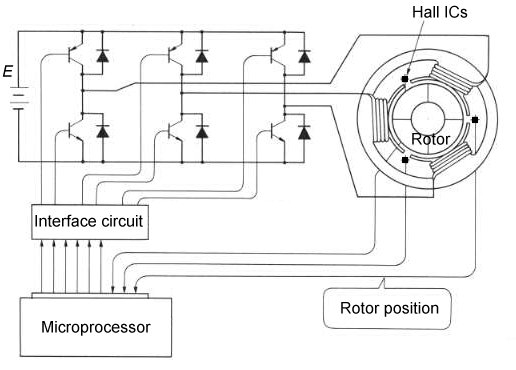
\includegraphics[width=10cm]{Images/inverter_1.png} 
\caption[Three-Phase Inverter]{Schematic representation of the three-phase inverter circuit needed to drive a brushless motor(\citeauthor{microchip}, \citeyear{microchip}).}
%http://www.ewh.ieee.org/soc/es/May2001/02/FIG2.JPG
\label{fig:inverter_1}
\end{figure}

The use of recirculation diodes is necessary to avoid damage in the transistors due to the overvoltage generated by the current transients in the windings $L dI/dt$ that takes place between the switches of a same branch of the inverter while switching from one state to another. For example, when a transistor is suddenly turned off, the current flowing through the coils doesn't instantly dissapear, but instead it recirculates through the diodes until it vanishes.

\subsection{Peripherals}




\section{PMAC Motors Driving Methods}\label{section:driving_methods}

\subsection{Trapezoidal Drive}

\subsection{Sinusoidal Drive}




\section{Control Methods}

\subsection{Speed Control}

\subsection{Torque Control}

\subsection{Field Oriented Control}

\subsection{Speed Control with Field Oriented Control}



 
	\chapter{Study Cases} \label{chap:robi}

(...)\\

\lipsum[1]

\section{Robi}

(...)\\

\lipsum[2]

\section{RC Vehicle}

(...)\\

\lipsum[3]
 
	\chapter{Project Development} \label{chap:implementation}

(...)\\

\section{Hypothesis}

(...)\\

\section{VESC Board}

The electric drive subject of this study is based on an open source project developed by the Swedish engineer Benjamin Vedder called VESC - Open Source ESC, which consists in the hardware design of a Printed Circuit Board (PCB) and the source code used to drive a BLDC motor.\\

The VESC board was conceived and designed to be used in electric skateboards with the intention to create one of the best electronic speed controllers available. Since it was planned to be used in a skateboard, it has a small form-factor and it can be used for different applications with similar power demand. The hardware can also be modified by changing specific components to drive motors with higher power demand or by modifying the PCB following the schematic design.

The board consists of the following blocks, which will be explained in detail in this chapter:
\begin {enumerate}
	\item Power supply input
	\item Power MOSFETs three-phase inverter
	\item MOSFET driver
	\item Microcontroller unit
	\item Peripherals
	\begin {aenumerate}
		\item Temperature sensors
		\begin {aenumerate}
			\item Motor temperature sensor
			\item Board temperature sensor
		\end {aenumerate}
		\item Hall effect sensors
		\item RC Servomotor Output
		\item Debug LEDs
	\end {aenumerate}
	\item Communication interfaces
	\begin {aenumerate}
		\item USB
		\item CAN
		\item USART
		\item SPI
		\item I2C
	\end {aenumerate}
\end {enumerate}

\subsection{Power Supply Input}
%The power is supplied into the board by means of soldering 2 wires into large pads placed closely to the three-phase inverter nodes V\_SUPPLY and GND. V\_SUPPLY and GND are the positive and negative nodes of the power supply source respectively. The power is supplied from a power regulator for static applications or from a battery for mobile applications. It is also specified that there should be a decoupling capacitor connected in parallel to the power supply port.\\

IMAGE\\

\subsubsection{Power Supply Range}
%he voltage range of the VESC board is defined by the MOSFET driver integrated circuit DRV8302, which specifies an operating supply voltage range from 8V to 60V, but allows a maximum voltage supply up to 65V (ref to the datasheet). All the other components of the board, mainly capacitors and power MOSFETs, must be selected according to this voltage range.\\

%The current range of the board is limited by the MOSFETs current limit and by the traces width in the PCB. This maximum values will be addressed later in the section dedicated to the power MOSFETs used in the board.\\

\subsubsection{Bulk Electrolytic Capacitor}
%It is important to place a bulk capacitance with an appropiate capacitance value and voltage range in parallel to the input of the power supply of a motor drive system. The main objective of a bulk capacitance is to control the voltage deviation at the input of a system when the converter is responding to an output load transient, meaning that if there is a load increase and the power supply is not able to provide the current instantaneously for the motor, the current must be provided by the bulk capacitor. The higher the capacitance at the input of the system, the lower the deviation at the load, but this comes at a cost of price and space, since the capacitance value of a capacitor is proportional to the size of its parallel plates. The value of the input bulk capacitor is determined mainly by the following factors:

\begin {enumerate}
	\item The largest amount of current required by the motor
	\item The capacitance of the power supply and its ability to source current
	\item The parasitic inductance between the power supply and the motor
	\item The acceptable voltage ripple
	\item The type of motor
\end {enumerate}

%The datasheet of a motor driver should generally provide a recommended value for the bulk capacitor, but it is necessary to calculate and test the value to determine if it's appropiate. The voltage rating of a bulk capacitor must be higher than the value of the power supply to provide a margin for cases in which the motor transfers energy to the supply, which would increase its voltage and would damage a capacitor with a smaller value than the resulting voltage.\\

%The magnitude of the input transient is calculated from equation XXX:\\

%FORMULA\\

%where n is efficiency, deltaiout is the output transient current, deltain is the input transient current, Vout is the nominal output voltage and vin is the nominal input voltage. After determining the input transient, we can calculate the capacitance value by using the following formula:\\

%FORMULA\\

%Since there is no filtering inductance in the system, we can consider a stray inductance of 50 nH in the calculation, obtaining a value of XXX uF for the bulk capacitance. By looking for commercially available capacitor values, we can round up the value of the capacitor to 2200uF and, considering the maximum input voltage value of the motors, we can double that value and define a voltage range of 70V, which is a commercially available value for a capacitor.\\

%It is important to note that since the value of this capacitance is large, also its size will be large, therefore it's important to consider its dimensions to setup a mechanically stable position for such capacitance with aims of avoiding hardware malfunction.\\ 

\subsubsection{Power Supply Wiring}
%The strategy of soldering the wires directly to the pads in the PCB helps reduce the size and price of the board since it avoids the use of large power traces in that would be needed if a regular receptacle connector was to be used.

%The practice of soldering a wire directly to a PCB is discouraged mainly in circuits that will be mounted in a system designed to be in movement (i.e. automotive or aerospace applications) because the wire used in these applications is made of delicate copper strands which can break easily with movement of the board or of the wires and cause a short circuit or a loose contact, both of which might lead to catastrophic failures (https://electronics.stackexchange.com/questions/129907/what-is-the-best-way-to-solder-these-wires-to-circuit-board), so there is a risk in this board since it will be mounted in systems that will be in constant movement (http://uk.rs-online.com/web/generalDisplay.html?id=solutions/pcb-connectors). Since this board was designed this way to reduce space consumption, the trade-off between safety and size was balanced into the size constraints, therefore some cautions must be taken to avoid problems, mainly because these wires carry a considerable amount of current and they pass over many components of the board as seen in figure X.

%The first consideration to be made is the wire gauge and insulation type. The wire gauge is a measurement of the wire diameter, which determines the amount of electric current that a wire can safely carry, as well as its electrical resistance and weight (http://en.wikipedia.org/wiki/Wire_gauge). Since the wire has an implicit resistance depending on its diameter as stated by Pouillets Law:\\

FORMULA\\

%where rho!!! is the electrical resistivity of the material, L is the length of the wire and A is the cross-sectional area of the wire (https://en.wikipedia.org/wiki/Electrical_resistivity_and_conductivity), there is also a voltage drop in the transmission line depending on the current flowing through the wire. This voltage drop can be neglected or not depending on the length of the wire being used, which defines 2 types of wiring: chassis wiring and transmission line wiring. For this board, it is suggested to use short wires to avoid a large voltage drop and to ease the handling of such wire until it reaches the output of the enclosure that will protect the circuit. In either case, the wire can be considered as chassis wiring since a transmission line wiring is considered for wires larger than 2 meters.\\

%The second consideration regarding the wire selection is the insulation material. Since the current passing through the copper also implies power consumption due to the resistance of the copper, there is heat transfer from the wire to its surroundings. To protect the copper strands from its surroundings and vice versa, wires are covered by an insulating material, which has low thermal and electrical conductivity.\\

%Since the heat exchange calculation of the wire would require many assumptions, it’s a normal practice to select the type of wire using tables that consider the temperature rise in the wire according to different currents and lengths. In the case of the PMSM motor used in Robi, the maximum current would be 13.88A, therefore we can use a table of wire gauges and currents under (…) (https://www.powerstream.com/Wire_Size.htm)\\

%RESULT OF THE CALCULATION\\

\subsection{Power MOSFET Three-Phase Inverter}
%The three-phase inverter used in the VESC board is based on the power MOSFET IRFS7530-7PPbF by the semiconductor company International Rectifier. \\

%IMAGE OF THE INVERTER\\

%This MOSFET is based on the HEXFET Power MOSFET technology, which is a Vertical Double-diffused MOS transistor (VDMOS) with hexagonal elementary cells in parallel which maximizes the W/L ratio of the transistor, reducing its on-resistance RDS(ON). (ref to Gionni and the datasheet).\\

%Image of the transistor

\subsubsection{Voltage and Current Limits}
%The DC Voltage limit in the inverter is defined by the drain-source breakdown voltage (V(BR)DSS) of the MOSFETs which is 60V\\

%SAY SOMETHING ABOUT THE CURRENT\\

%INCLUDE TABLE WITH ABSOLUTE VALUES\\

\subsubsection{Switching Times}

%(...)\\


\subsection{MOSFET Driver}
%The central component in the VESC board around which the rest of the circuit was designed is the integrated circuit DRV8302, a brushless motor inverter driver manufactured by Texas Instruments.\\

%INCLUDE SIMPLIFIED SCHEMATIC DIAGRAM OF THE DRIVER\\

%The DRV8302 provides three half bridge drivers capable of driving two N-channel MOSFETs each. (...)\\

%The device supports up to 1.7-A source and 2.3-A peak current capability. (...)\\

%The DRV8302 can operate off of a single power supply with a wide range from 8-V to 60-V. (...)\\

%It uses a bootstrap gate driver architecture with trickle charge circuitry to support 100 duty cycle. (...)\\

%The DRV8302 uses automatic hand shaking when the high side or low side MOSFET is switching to prevent current shoot through. (...)\\

%Integrated VDS sensing of the high and low side MOSFETs is used to protect the external power stage against overcurrent conditions. (...)\\

%The DRV8303 includes two current shunt amplifiers for accurate current measurement. The amplifiers support bi-directional current sensing and provide and adjustable output offset up to 3 V. (...)\\

%The DRV8302 also includes an integrated switching mode buck converter with adjustable output and switching frequency. The buck converter can provide up to 1.5 A to support MCU or additional system power needs. (...)\\

%A hardware interface allows for configuring various device parameters including dead time, overcurrent, PWM mode, and amplifier settings. Error conditions are reported through the nFAULT and nOCTW pins. 3.3-V and 5-V Interface Support. (...)\\


\subsection{Microcontroller Unit}

%The processor for which this board was designed is the STM32F405rg: a 64-pin IC microcontroller of the STMicroelectronics family of 32-bit devices with an ARM Cortex-M4 CPU and a core operating frequency up to 168 MHz. The Cortex-M4 core features a Floating point unit (FPU) single precision which supports all ARM single-precision data-processing instructions and data types. It also implements a full set of DSP instructions, which makes it ideal for the signal processing required to drive PMAC motors. This microcontroller also includes three 12-bit ADCs and supports USART, I2C, SPI, USB and CAN communication interfaces, improving the versatility of the VESC board. The memory of the microcontroller consists in 1024 kB of Flash memory and 192 kB of SRAM memory.\\

High-performance MCUs with DSP and FPU instructions
ARM Cortex-M4-based
Up to 180 MHz operating frequency
Up to 2 Mbytes Flash
Up to 384 kB RAM
Ethernet IEEE 1588
SDIO
16 and 32-bit timers
2 CAN ports
Camera
SDRAM
SPI
12-bit DAC and ADC
USB 2.0 OTG


\subsection{PCB Layout}

(...)\\

\lipsum[8]

\section{Measurement Board}

(...)\\

\lipsum[9]

\subsection{Voltage Measurement}

(...)\\

\lipsum[10]

\subsection{Current Measurement}

(...)\\

\lipsum[11]

\subsection{Data acquisition}

(...)\\

\lipsum[12]

\section{Angular Position Sensor}

(...)\\

\lipsum[13]

\section{Miosix}

(...)\\

\lipsum[14]

\section{Test Setup}

(...)\\

\lipsum[15]

\subsection{Robi Setup}

(...)\\

\lipsum[16]

\subsubsection{Marelli Generator as Load}

(...)\\

\lipsum[17]

\subsection{RC Vehicle Setup}

(...)\\

\lipsum[18]

\section{Algorithms Implementation}

(...)\\

\lipsum[19]

\subsection{6-Step Drive Implementation}

(...)\\

\lipsum[20]

\subsection{Field Oriented Control Implementation}

(...)\\

\lipsum[21]

\section{Simulation?}

(...)\\

\lipsum[22]







 
	\chapter{Results} \label{chap:results}

(...)\\

\lipsum[1]

\section{BLDC}

(...)\\

\lipsum[2]

\subsection{Voltage Waveforms}

(...)\\

\lipsum[3]

\subsection{Current Waveforms}

(...)\\

\lipsum[4]

\subsection{Voltage Control Plots}

(...)\\

\lipsum[5]

\subsection{Current Control Plots}

(...)\\

\lipsum[6]

\section{PMSM}

(...)\\

\lipsum[7]

\subsection{Voltage Waveforms}

(...)\\

\lipsum[8]

\subsection{Current Waveforms}

(...)\\

\lipsum[9]

\subsection{Voltage Control Plots}

(...)\\

\lipsum[10]

\subsection{Current Control Plots}

(...)\\ 
	\chapter{Conclusion} \label{chap:conclusion}

(...)\\

\lipsum[1]

\section{Bla bla bla}

(...)\\

\lipsum[2]

\section{Future Work}

(...)\\

\lipsum[3]
 
		
	% ************************************************************
	% Backmatter
	%*************************************************************
	\cleardoublepage%********************************************************************
% Bibliography
%*******************************************************
% work-around to have small caps also here in the headline
\manualmark
\markboth{\spacedlowsmallcaps{\bibname}}{\spacedlowsmallcaps{\bibname}}
%\phantomsection 
\refstepcounter{dummy} 
% to have the bib a bit from the rest in the toc
\addtocontents{toc}{\protect\vspace{\beforebibskip}}
\addcontentsline{toc}{chapter}{\tocEntry{\bibname}}
\label{app:bibliography} 
\printbibliography
	\appendix
	% \cleardoublepage\part{Appendix}
	%********************************************************************
% Appendix
%*******************************************************
% If problems with the headers: get headings in appendix etc. right
\markboth{\spacedlowsmallcaps{Appendix}}{\spacedlowsmallcaps{Appendix}}
%************************************************
\chapter{Appendix example: code listings}

\begin{flushright}{\slshape    
    We have seen that computer programming is an art, \\ 
    because it applies accumulated knowledge to the world, \\ 
    because it requires skill and ingenuity, and especially \\
    because it produces objects of beauty.} \\ \medskip
    --- \citeauthor{knuth:1974}, \citetitle{knuth:1974},
\citeyear{knuth:1974} 
\end{flushright}

\section{The \texttt{listings} package to include source code}
Source code is usually not part of the text of a thesis, but if it is an original contribution it makes sense to le the code speak by itself instead of describing it. The package \verb!listings! provide the proper layout tools. Refer to its manual if you need to use it, an example is given in listing \ref{lst:probCounter}.

\lstinputlisting[
	firstline=1,
	lastline=47,
	float=tb,
	language=C++,
	tabsize=2,
	numbers=left,
	numberstyle=\tiny,
	stepnumber=2,
	numbersep=5pt,
	caption={Code snippet with the recursive function to evaluate the pdf of the sum $Z_N$ of $N$ random variables equal to $X$.}, 
	captionpos=t,
	label=lst:probCounter
	]{CodeFiles/probabilityCounter.cpp}

\end{document}
% ****************************************************************